\documentclass[a4paper,11pt,twoside,openright]{book}

\usepackage{makeidx}
\usepackage{amsmath}
\usepackage{amssymb}
\usepackage{amsthm}
\usepackage{graphicx}
\usepackage{longtable}
\usepackage{tablefootnote}
% adjust the width of caption in longtable
\setlength{\LTcapwidth}{1.3\textwidth}
\usepackage{lscape}
% change "blue" to "black" if printted
\usepackage[pdftex,draft=false,colorlinks=true,bookmarksnumbered=true,
            hyperindex,pdfstartview=FitH,plainpages=false,
            linkcolor=blue,citecolor=blue,urlcolor=blue]{hyperref}
%CJKbookmarks=true
\usepackage[square,comma,numbers,sort&compress]{natbib}
\usepackage{hypernat}
%\usepackage{citesort}  %sort citations
\usepackage[T1]{fontenc} %make nice pdf on screen
% leave space around whole list
\usepackage{enumitem}
\setlist{nolistsep}

% indexing
\usepackage{makeidx}

\usepackage{pgfplots}

% used for notice, remove this at the end
\usepackage{xcolor}
\newcommand{\fixme}[1]{\textbf{\textit{\color{red} #1}}}

% page layout
\setlength{\marginparwidth}{0in}
\setlength{\evensidemargin}{-0.4in}
\setlength{\oddsidemargin}{-0.07in} 
\setlength{\textwidth}{6.76in}
\setlength{\topmargin}{0in}
\setlength{\textheight}{9in}

% all the figures are in directory "figures"
\graphicspath{{figures/}}

% footnote style
%\renewcommand{\thefootnote}{\fnsymbol{footnote}}

% indexing
\makeindex

\begin{document}

% front matter
\frontmatter
\pagestyle{empty}

% title page
\vspace*{\fill}
\begin{center}
  \begin{Huge}\textsf{{\huge QcMatrix}}\end{Huge}\\[0.5\baselineskip]
  \begin{LARGE}\textsf{Version 0.1.0}\end{LARGE}
\end{center}

\vspace*{\fill}
\begin{center}
  \begin{huge}\textsf{Bin Gao}\end{huge}\\[0.5\baselineskip]
  \begin{LARGE}\textsf{\today}\end{LARGE}
\end{center}

\vspace*{\fill}
\begin{center}
  \begin{large}
    \textsf{Centre for Theoretical and Computational Chemistry (CTCC)}\par
    \textsf{Department of Chemistry}\par
    \textsf{University of Troms{\o} --- The Arctic University of Norway}\par
    \textsf{N--9037, Troms{\o}, Norway}\\[0.5\baselineskip]
  \end{large}
\end{center}

\clearpage

% copyright page
\begingroup
\footnotesize
\setlength{\parindent}{0pt}
\setlength{\parskip}{\baselineskip}
\textcopyright{} 2010~--~2015 Bin Gao\\

\textsc{QcMatrix} is free software: you can redistribute it and/or modify
it under the terms of the GNU Lesser General Public License as published by
the Free Software Foundation, either version 3 of the License, or
(at your option) any later version.

\textsc{QcMatrix} is distributed in the hope that it will be useful,
but WITHOUT ANY WARRANTY; without even the implied warranty of
MERCHANTABILITY or FITNESS FOR A PARTICULAR PURPOSE. See the
GNU Lesser General Public License for more details.

You should have received a copy of the GNU Lesser General Public License
along with \textsc{QcMatrix}. If not, see\linebreak \url{http://www.gnu.org/licenses/}.
\endgroup
\clearpage

% contents
\pagestyle{headings}

%\makeindex

\tableofcontents

% preface
%\chapter*{Preface}
%\label{chapter-preface}
%
%\addcontentsline{toc}{chapter}{Preface}

% acknowledgments
%\chapter*{Acknowledgments}
%\label{chapter-acknowledgments}
%
%\addcontentsline{toc}{chapter}{Acknowledgments}

% body
\mainmatter
\pagenumbering{arabic}

% introduction of QcMatrix
\chapter{What is \textsc{QcMatrix}?}
\label{chapter-introduction}

\textsc{QcMatrix} is an ``abstract'' matrix library written in C language (with C++
and Fortran interface), and provides a ``speical'' square block complex matrix (as
shown in Fig.~\ref{fig-block-cmplx} and see the discussion below) and corresponding
functions.
\begin{figure}[htbp]
  \centering
  \includegraphics[width=10cm]{block_cmplx.pdf}
  \caption{Illustration of the square block complex matrix implemented in
    \textsc{QcMatrix}~---~$4\times 4$ blocks, with red blocks as the non-zero
    complex matrices. Each block is square matrix with the same dimension.}
  \label{fig-block-cmplx}
\end{figure}

\noindent In general, a square block matrix $\mathbf{A}$ satisfies\cite{Schaum-Linear-Algebra}:
\begin{enumerate}
  \item $\mathbf{A}$ is a square matrix,
  \item the blocks form a square matrix,
  \item the diagonal blocks are also square matrices;
\end{enumerate}
for instance, a $N\times N$ square block matrix $\mathbf{A}$ takes the following structure
\begin{equation}
  \mathbf{A}=%
  \begin{bmatrix}
    \mathbf{A}_{11} & \mathbf{A}_{12} & \cdots & \mathbf{A}_{1N}\\
    \mathbf{A}_{21} & \mathbf{A}_{22} & \cdots & \mathbf{A}_{2N}\\
    \cdots & \cdots & \cdots & \cdots\\
    \mathbf{A}_{N1} & \mathbf{A}_{N2} & \cdots & \mathbf{A}_{NN}
  \end{bmatrix},
\end{equation}
where $\mathbf{A}_{II}$ ($1\le I\le N$) is also square matrix ($\mathbf{A}_{I\ne J}$
may not be square matrix).

The square block complex matrix implemented in \textsc{QcMatrix} is a special square block
matrix that we also require \textbf{all the blocks have the same dimension}\footnote{So all
the blocks are square matrix with the same dimension.}. As shown in Fig.~\ref{fig-block-cmplx},
in the \textsc{QcMatrix} library, the square block complex matrix and its operations at the
block level are taken care by the codes in \verb|src/qcmat| directory, while the complex
matrix of each non-zero block (zero blocks denoted as \verb|QNULLMAT|, will not participate
in the matrix operations) and its operations are carried out by the codes in \verb|src/cmplx_mat|
directory.

As an ``abstract'' matrix library, \textsc{QcMatrix} should be in general built on top of
external matrix library, which is written either in C, C++ or Fortran language. As illustrated
in Fig.~\ref{fig-lang-adapter}, \textsc{QcMatrix} can be viewed as an adapter between external
matrix libraries and application libraries (which depends on the matrix and matrix operations)
written in different languages~---~C, C++ or Fortran. The conversion between different languages
is taken care by \textsc{QcMatrix}, so that the application libraries can in principle, without
any modification, use different external matrix libraries through the \textsc{QcMatrix}.
\begin{figure}[htbp]
  \centering
  \includegraphics[width=8cm]{lang_adapter.pdf}
  \caption{\textsc{QcMatrix} as an adapter between different languages.}
  \label{fig-lang-adapter}
\end{figure}

\textsc{QcMatrix} can also work as an adapter between different matrices. As shown in
Fig.~\ref{fig-matrix-adapter}, whatever implemented in the external library~---~real
matrix, complex matrix, square block real matrix or square block complex matrix~---~can
all be ``translated'' by \textsc{QcMatrix}, which then provides the square block complex
matrix to different application libraries.
\begin{figure}[htbp]
  \centering
  \includegraphics[width=9cm]{matrix_adapter.pdf}
  \caption{\textsc{QcMatrix} as an adapter between different matrices.}
  \label{fig-matrix-adapter}
\end{figure}

The application programming interface (API) of \textsc{QcMatrix} for different languages
is slight different. For instance, including \textsc{QcMatrix} in a code and declaration
of a matrix are a bit different in different languages, as illustrated in Table~\ref{tab-QcMatrix-use}.
Details of the \textsc{QcMatrix} APIs are given in Chapter~\ref{chapter-API}.
\begin{table}[hbtp]
  \centering
  \caption{Using \textsc{QcMatrix} in different languages\index{\textsc{QcMatrix} APIs}.}
  \label{tab-QcMatrix-use}
  \begin{tabular}{l|l|l}
    \hline\hline
    \textbf{Language} & \textbf{Including \textsc{QcMatrix}} & \textbf{Declaration of a matrix}\\
    \hline
    C & \verb|#include "qcmatrix.h"| & \verb|QcMat A;|\\
    \hline
    C++ & &\\
    \hline
    Fortran & \verb|use qcmatrix_f| & \verb|type(QcMat) A|\\
    \hline\hline
  \end{tabular}
\end{table}

To use \textsc{QcMatrix}, the external library should also implement the matrix type
and functions/subroutines required by \textsc{QcMatrix}. Detailed information can be
found in Chapter~\ref{chapter-external-lib}, we give in Table~\ref{tab-external-req}
the required header files/modules and implemented matrix type in the external library.
\begin{table}[hbtp]
  \centering
  \caption{Required header files/modules and implemented matrix in the external
    library\index{Requisite for external library}.}
  \label{tab-external-req}
  \begin{tabular}{l|l|l}
    \hline\hline
    \textbf{Language} & \textbf{Header file/Module} & \textbf{Implemented matrix}\\
    \hline
    C & \verb|LANG_C_HEADER| & \verb|struct LANG_C_MATRIX|\\
    \hline
    C++ & &\\
    \hline
    Fortran & \verb|LANG_F_MODULE| & \verb|type LANG_F_MATRIX|\\
    \hline\hline
  \end{tabular}
\end{table}

The left chapters in this manual are: Chapter~\ref{chapter-installation} describes the
installation and test suite of \textsc{QcMatrix},
Chapters~\ref{chapter-SCF-solvers}--\ref{chapter-molecular-electronics} are the applications
built on top of the \textsc{QcMatrix} library, respectively, the self-consistent field
solvers (Chapter~\ref{chapter-SCF-solvers}), linear response solvers (Chapter~\ref{chapter-RSP-solvers}),
simulations of X-ray spectroscopies (Chapter~\ref{chapter-xray}) and molecular electronics
(Chapter~\ref{chapter-molecular-electronics}). Chapter~\ref{chapter-QcMatrix-advanced}
contains some advanced topics of \textsc{QcMatrix}, which may be only relevant for
\textsc{QcMatrix} developers. Finally, Chapters~\ref{chapter-files} and \ref{chapter-limitations}
respectively describe the files and directories of \textsc{QcMatrix}, and some limitations
of \textsc{QcMatrix}.

If there is any question regarding the use of \textsc{QcMatrix}, please contact the authors
in the file \verb|AUTHORS|. If you have used \textsc{QcMatrix} and found it is useful, please
consider to cite \textsc{QcMatrix} as
\begin{verbatim}
    @misc{QcMatrix,
      author = {Bin Gao},
      title = {{QcMatrix Version 0.1.0}},
      year = {2015},
      note = {https://gitlab.com/bingao/qcmatrix}
    }
\end{verbatim}

\chapter{Installation}
\label{chapter-installation}

Before installing \textsc{QcMatrix}, you need to make sure the following programs are
installed on your computer:
\begin{enumerate}
  \item Git,
  \item CMake ($\ge2.8$),
  \item HDF 5 ($\ge1.8$) if matrix I/O is enabled (if HDF 5 is not available, ordinary
    binary format file will be used which is not portable),
  \item C, C++ (if C++ adapter and APIs required) and/or Fortran (if Fortran adapter
    and APIs needed) compilers,
  \item BLAS and LAPACK libraries for test suite and/or \textsc{QcMatrix} internal real
    matrix library.
\end{enumerate}

\textsc{QcMatrix} can be got as:
\begin{verbatim}
    git clone git@gitlab.com:bingao/qcmatrix.git
\end{verbatim}
Afterwards, you could start to compile \textsc{QcMatrix}.

\section{CMake}
\label{section-install-cmake}

For the time being, only CMake could be used to compile \textsc{QcMatrix}. In general,
\textsc{QcMatrix} should be compiled together with the external libraries or host
programs. See for example the \textsc{Dalton} program\footnote{Currently,
\textsc{QcMatrix} is implemented in the \texttt{qcmatrix} branch of \textsc{Dalton}
program. Interested users could check these directories in \textsc{Dalton}:
\texttt{DALTON/qcmatrix} and \texttt{LSDALTON/qcmatrix}.}.

If there is no external library, you could still compile \textsc{QcMatrix} by (i) using
its own internal real matrix library (in \verb|src/real_mat|, may not be efficient), or
(ii) using the simple C++ or Fortran matrix libraries in \verb|tests/cxx/adapter| and
\verb|tests/f90/adapter|\footnote{In that case, you first need to compile the C++ or
Fortran matrix libraries. Please follow the \texttt{README} file therein.}. Let us
assume that you want to compile the library in directory \verb|build|, you could
invoke the following commands:
\begin{verbatim}
    mkdir build
    cd build
    ccmake ..
    make
\end{verbatim}
During the step \verb|ccmake|, you need to set some parameters appropriately for the
compilation. For instance, if you enable \verb|QCMATRIX_TEST_EXECUTABLE|, some executables
for the test suite will be built and can run after compilation. So that you are able to
check if \textsc{QcMatrix} has been successfully compiled. A detailed list of the parameters
controlling the compilation is given in Table~\ref{tab-cmake-parameters}.
\begin{center}
  \begin{longtable}{l|p{0.42\textwidth}|l}
    \caption{CMake parameters controlling the compilation of \textsc{QcMatrix}\index{CMake parameters}.}
    \label{tab-cmake-parameters}\\
% this is the header for the first page of the table
    \hline\hline
    \textbf{Parameter} & \textbf{Description} & \textbf{Default}\\
    \hline
    \endfirsthead
% this is the header for the remaining page(s) of the table
    \multicolumn{3}{c}{{\bfseries \tablename\ \thetable{} -- continued from previous page}}\\
    \hline\hline
    \textbf{Parameter} & \textbf{Description} & \textbf{Default}\\
    \hline
    \endhead
% this is the footer for all pages except the last page of the table
    \hline
    \multicolumn{3}{r}{Continued on next page}\\
    \hline
    \endfoot
% this is the footer for the last page of the table
    \hline\hline
    \endlastfoot
%
    \verb|QCMATRIX_3M_METHOD| & Enable 3M method for complex matrix-matrix multiplication. & \verb|ON|\\
    \verb|QCMATRIX_64BIT_INTEGER| & Use 64 bit integer. & \verb|OFF|\\
    \verb|QCMATRIX_AUTO_ERROR_EXIT|\footnote{If \texttt{QCMATRIX\_AUTO\_ERROR\_EXIT=ON},
                                            \textsc{QcMatrix} will automatically exit on error,
                                            and users can not check the return error information.} %
      & Enable automatic exit on error. & \verb|OFF|\\
    \verb|QCMATRIX_BLAS_64BIT| & Use 64 bit BLAS and LAPACK libraries. & \verb|OFF|\\
    \verb|QCMATRIX_ENABLE_VIEW| & Enable matrix I/O. & \verb|OFF|\\
    \verb|QCMATRIX_ENABLE_HDF5|  & Enable the use of HDF5 library for matrix I/O. & \verb|ON|\\
    \verb|QCMATRIX_SINGLE_PRECISION| & Use single precision for real numbers. & \verb|OFF|\\
    \verb|QCMATRIX_STORAGE_MODE| & Enable different matrix storage modes. & \verb|OFF|\\
    \verb|QCMATRIX_STRASSEN_METHOD| %
      & Strassen's method for the square block complex matrix-matrix multiplication. & \verb|ON|\\
    \verb|LIB_QCMATRIX_NAME| & Sets the name of the QcMatrix library. & \verb|qcmatrix|\\
    \verb|QCMATRIX_ROW_MAJOR|\footnote{The column major order is recommended if \textsc{QcMatrix}
                                    internal real matrix library is used (i.e., if
                                    \texttt{BUILD\_ADAPTER=OFF}).} %
      & Row major order for matrix elements. & \verb|OFF|\\
    \verb|QCMATRIX_ZERO_BASED|\footnote{\texttt{QCMATRIX\_SINGLE\_PRECISION},
                                         \texttt{QCMATRIX\_ROW\_MAJOR} and
                                         \texttt{QCMATRIX\_ZERO\_BASED} should
                                         be consistent with external matrix library
                                         if \texttt{BUILD\_ADAPTER=ON}.} %
      & Zero-based numbering. & \verb|ON|\\
    \hline
    \textbf{Adapter} & &\\
    \verb|QCMATRIX_BUILD_ADAPTER| & Build the adapter for external matrix library. & \verb|OFF|\\
    \verb|QCMATRIX_ADAPTER_TYPE| %
      & Choose the type of the external library, valid entries are \verb|C;CXX;F90;F03|. & \verb|C|\\
    \verb|EXTERNAL_BLOCK_MATRIX| & Square block matrix implemented in the external library. & \verb|OFF|\\
    \verb|EXTERNAL_COMPLEX_MATRIX| & Complex matrix implemented in the external library. & \verb|OFF|\\
    \verb|QCMATRIX_EXTERNAL_LIBRARIES| %
      & Sets the external libraries for QcMatrix (like \verb|-lxxxx|). & \verb|None|\\
    \verb|QCMATRIX_EXTERNAL_PATH| & Sets the path of external libraries for QcMatrix. & \verb|None|\\
    \hline
    \textbf{Adapter (C)} & &\\
    \verb|LANG_C_HEADER| & Name of header file of the external C library. & \verb|lib_matrix.h|\\
    \verb|LANG_C_MATRIX| & Name of external C matrix struct. & \verb|matrix_t|\\
    \hline
    \textbf{Adapter (F90)} & &\\
    \verb|LANG_F_MATRIX| & Name of external Fortran 90 matrix type. & \verb|matrix_t|\\
    \verb|LANG_F_MODULE| & Name of external Fortran 90 matrix module. & \verb|lib_matrix|\\
    \verb|SIZEOF_F_TYPE_P| %
      & Size (in bytes) of Fortran 90 derived types with a single pointer member. & \verb|12|\\
    \hline
    \textbf{Adapter (F03)} & &\\
    \verb|LANG_F_MATRIX| & Name of external Fortran 2003 matrix type. & \verb|matrix_t|\\
    \verb|LANG_F_MODULE| & Name of external Fortran 2003 matrix module. & \verb|lib_matrix|\\
    \hline
    \textbf{API} & &\\
    \verb|QCMATRIX_CXX_API| & Build C++ API. & \verb|OFF|\\
    \verb|QCMATRIX_Fortran_API| & Build Fortran API, options are: \verb|None;F90;F03|. & \verb|None|\\
    \hline
    \textbf{Matrix I/O} & &\\
    \verb|HDF5_DIR| %
      & The directory containing a CMake configuration file for HDF5. & \verb|HDF5_DIR-NOTFOUND|\\
    \verb|HDF5_ROOT| & Provide a hind about where to find the HDF5 installation. & \verb|None|\\
    \verb|HDF5_USE_STATIC_LIBRARIES| & Enable the static link for HDF5. & \verb|ON|\\
    \hline
    \textbf{Test suite} & &\\
    \verb|QCMATRIX_TEST_3M_METHOD| & Build the test of efficiency of 3M method. & \verb|OFF|\\
    \verb|QCMATRIX_TEST_EXECUTABLE| & Build the test suite excutables. & \verb|ON|\\
  \end{longtable}
\end{center}
\vspace*{-5ex}

If no error happened, you will have a library named \verb|lib${LIB_QCMATRIX_NAME}.a|,
where\linebreak \verb|LIB_QCMATRIX_NAME| is set during CMake procedure.

\section{Test Suite}
\label{section-test-suite}

All the tests are in the directory \verb|tests|, and will also be compiled.
As aforementioned, these tests will be built as executables if
\verb|QCMATRIX_TEST_EXECUTABLE| is enabled (more explicitly,
\verb|${LIB_QCMATRIX_NAME}_c_test| will always be built,
\verb|${LIB_QCMATRIX_NAME}_cxx_test| and \verb|${LIB_QCMATRIX_NAME}_f_test|
will be built only if C++ and Fortran APIs are built). Otherwise, these
tests will be compiled and into the library \verb|lib${LIB_QCMATRIX_NAME}.a|
so that they could be invoked from the host program as,\linebreak
\verb|ierr = test_c_QcMatrix()| (C and C++) or \verb|call test_f_QcMatrix(io_log)|
(Fortran).

In most tests, we compare the results from \textsc{QcMatrix} and those from the
BLAS and/or LAPACK routines by using the whole matrix as an array.

% API references
\chapter{\textsc{QcMatrix} API Reference\index{\textsc{QcMatrix} APIs}}
\label{chapter-API}

As mentioned in Chapter~\ref{chapter-introduction}, the API of \textsc{QcMatrix} is only
slight different for different languages. Including \textsc{QcMatrix} in a code and
declaration of a matrix has been given in Table~\ref{tab-QcMatrix-use}. In this chapter,
we will describe the \textsc{QcMatrix} API references in detail.

First, there are some parameters defined in \textsc{QcMatrix} that can be used by users,
as given in Table~\ref{tab-QcMatrix-parameters}.
\begin{center}
  \small
  \begin{longtable}{l|l|p{0.5\textwidth}}
    \caption{Public parameters provided by \textsc{QcMatrix}\index{\textsc{QcMatrix} parameters}.}
    \label{tab-QcMatrix-parameters}\\
% this is the header for the first page of the table
    \hline\hline
    \textbf{Parameter} & \textbf{Type} & \textbf{Description}\\
    \hline
    \endfirsthead
% this is the header for the remaining page(s) of the table
    \multicolumn{3}{c}{{\bfseries \tablename\ \thetable{} -- continued from previous page}}\\
    \hline\hline
    \textbf{Parameter} & \textbf{Type} & \textbf{Description}\\
    \hline
    \endhead
% this is the footer for all pages except the last page of the table
    \hline
    \multicolumn{3}{r}{Continued on next page}\\
    \hline
    \endfoot
% this is the footer for the last page of the table
    \hline\hline
    \endlastfoot
%
    \verb|QSUCCESS| & \verb|QErrorCode| & Function returns no error.\\
    \verb|QFAILURE| & \verb|QErrorCode| & Function returns with error.\\
    \verb|QTRUE| & \verb|QBool| & Boolean type, true.\\
    \verb|QFALSE| & \verb|QBool| & Boolean type, false.\\
    \verb|QZEROTHRSH| & \verb|QReal| & Threshold for nearly negligible number.\\
    \verb|QSYMMAT| & \verb|QcSymType| & Symmetric (Hermitian) matrix.\\
    \verb|QANTISYMMAT| & \verb|QcSymType| & Anti-symmetric (anti-Hermitian) matrix.\\
    \verb|QNONSYMMAT| & \verb|QcSymType| & Non-symmetric (non-Hermitian) matrix.\\
    \verb|QNULLMAT| & \verb|QcDataType| & Matrix that neither real nor imaginary part is assembled.\\
    \verb|QREALMAT| & \verb|QcDataType| & Real matrix.\\
    \verb|QIMAGMAT| & \verb|QcDataType| & Imaginary matrix.\\
    \verb|QCMPLXMAT| & \verb|QcDataType| & Complex matrix.\\
    \verb|UNKNOWN_STORAGE_MODE|\footnote{Available if \texttt{QCMATRIX\_STORAGE\_MODE} is set in CMake.} %
      & \verb|QcStorageMode| %
      & Unknown storage mode (mostly for error handling), while specific storage modes
        should be defined and implemented in the external library.\\
    \verb|COPY_PATTERN_ONLY| & \verb|QcDuplicateOption| %
      & Duplicate option, copies the pattern of a matrix only (previous numerical values
        may be removed depending on the external library).\\
    \verb|COPY_PATTERN_AND_VALUE| & \verb|QcDuplicateOption| %
      & Duplicate option, copies an entire matrix including its numerical values.\\
    \verb|MAT_NO_OPERATION| & \verb|QcMatOperation| & No matrix operation performed.\\
    \verb|MAT_TRANSPOSE| & \verb|QcMatOperation| & Transpose.\\
    \verb|MAT_HERM_TRANSPOSE| & \verb|QcMatOperation| & Hermitian transpose.\\
    \verb|MAT_COMPLEX_CONJUGATE| & \verb|QcMatOperation| & Complex conjugate.\\
    \verb|BINARY_VIEW|\footnote{Both \texttt{BINARY\_VIEW} and \texttt{ASCII\_VIEW}
                                are available if \texttt{QCMATRIX\_ENABLE\_VIEW} is set in CMake.} %
      & \verb|QcViewOption| & Reads/writes a matrix in file using binary format.\\
    \verb|ASCII_VIEW| & \verb|QcViewOption| & Reads/writes a matrix in file using ASCII format.\\
  \end{longtable}
\end{center}
\vspace*{-5ex}

For Fortran users, the types in Table~\ref{tab-QcMatrix-parameters} are different.
Please refer to Table~\ref{tab-Fortran-types} for the convention of types in Fortran.
\begin{table}[hbtp]
  \centering
  \caption{Fortran type conventions\index{Fortran type conventions}.}
  \label{tab-Fortran-types}
  \begin{tabular}{l|l}
    \hline\hline
    \textbf{Type in \textsc{QcMatrix}} & \textbf{Fortran}\\
    \hline
    \verb|struct QcMat| & \verb|type(QcMat)|\\
    \verb|QErrorCode| & \verb|integer|\\
    \verb|QChar| & \verb|character*(*)|\\
    \verb|QInt| & \verb|integer|\\
    \verb|QBool| & \verb|logical|\\
    \verb|QReal| & \verb|real(QREAL)|\tablefootnote{\texttt{QReal} and \texttt{QREAL}
                                                    are the type of real numbers,
                                                    determined by \texttt{QCMATRIX\_SINGLE\_PRECISION}
                                                    during setting up CMake.}\\
    \verb|QcDataType| & \verb|integer|\\
    \verb|QcDuplicateOption| & \verb|integer|\\
    \verb|QcMatOperation| & \verb|integer|\\
    \verb|QcStorageMode| & \verb|integer|\\
    \verb|QcSymType| & \verb|integer|\\
    \verb|QcViewOption| & \verb|integer|\\
    \hline\hline
  \end{tabular}
\end{table}

The functions provided by \textsc{QcMatrix} are listed in Table~\ref{tab-QcMat-public-fun},
in which
\begin{enumerate}
  \item All functions are implemented in the directory \verb|src/qcmat|.
  \item All functions should be used as \verb|ierr = QcMat...(...)|, where
    \verb|QErrorCode ierr| contains the error information. It should be
    \verb|QSUCCESS| if no error happened.
  \item All matrices must first be created by calling \verb|QcMatCreate|,
    and finally destroyed by calling \verb|QcMatDestroy|. Futher requirements
    could be needed for some functions (for instance, the matrix should be
    assembled by calling \verb|QcMatAssemble|), please check the description
    of the functions in Table~\ref{tab-QcMat-public-fun}.
  \item All functions can be used in the same way in Fortran code, but the types
    of some arguments are different from those in C/C++ code, please refer to
    Table~\ref{tab-Fortran-types} for the convention of types in Fortran.
\end{enumerate}

\begin{center}
  \small
  \begin{longtable}{l|p{0.5\textwidth}}
    \caption{Public functions provided by \textsc{QcMatrix}\index{\textsc{QcMatrix} functions}.}
    \label{tab-QcMat-public-fun}\\
% this is the header for the first page of the table
    \hline\hline
    \textbf{Function/Arguments} & \textbf{Description}\\
    \hline
    \endfirsthead
% this is the header for the remaining page(s) of the table
    \multicolumn{2}{c}{{\bfseries \tablename\ \thetable{} -- continued from previous page}}\\
    \hline\hline
    \textbf{Function/Arguments} & \textbf{Description}\\
    \hline
    \endhead
% this is the footer for all pages except the last page of the table
    \hline
    \multicolumn{2}{r}{Continued on next page}\\
    \hline
    \endfoot
% this is the footer for the last page of the table
    \hline\hline
    \endlastfoot
%
    \verb|QcMatCreate|\index{\texttt{QcMatCreate}} %
      & Creates the context of a matrix.\\
    \hspace*{2ex}\verb|QcMat *A| %
      & \textsl{Input \& output}, the matrix.\\
    \hline
%
    \verb|QcMatBlockCreate|\index{\texttt{QcMatBlockCreate}} %
      & Sets the dimension of blocks and creates the blocks.\\
    \hspace*{2ex}\verb|QcMat *A| %
      & \textsl{Input \& output}, the matrix, should be created by \verb|QcMatCreate|.\\
    \hspace*{2ex}\verb|const QInt dim_block| %
      & \textsl{Input}, the dimension of blocks.\\
    \hline
%
    \verb|QcMatSetSymType|\index{\texttt{QcMatSetSymType}} %
      & Sets the symmetry type of a matrix.\\
    \hspace*{2ex}\verb|QcMat *A| %
      & \textsl{Input \& output}, the matrix, should be created by \verb|QcMatCreate|
        and \verb|QcMatBlockCreate|.\\
    \hspace*{2ex}\verb|const QcSymType sym_type| %
      & \textsl{Input}, given symmetry type, see file \verb|include/types/mat_symmetry.h|.\\
    \hline
%
    \verb|QcMatSetDataType|\index{\texttt{QcMatSetDataType}} %
      & Sets the data types of matrix elements of some blocks.\\
    \hspace*{2ex}\verb|QcMat *A| %
      & \textsl{Input \& output}, the matrix, should be created by \verb|QcMatCreate|
        and \verb|QcMatBlockCreate|.\\
    \hspace*{2ex}\verb|const QInt num_blocks| %
      & \textsl{Input}, number of blocks to set the data types.\\
    \hspace*{2ex}\verb|const QInt idx_block_row[]| %
      & \textsl{Input}, row indices of the blocks.\\
    \hspace*{2ex}\verb|const QInt idx_block_col[]| %
      & \textsl{Input}, column indices of the blocks.\\
    \hspace*{2ex}\verb|const QcDataType block_data_types[]| %
      & \textsl{Input}, given data types of the blocks, see file
        \verb|include/types/mat_data.h|.\\
    \hline
%
    \verb|QcMatSetDimMat|\index{\texttt{QcMatSetDimMat}} %
      & Sets the dimension of each block of a matrix.\\
    \hspace*{2ex}\verb|QcMat *A| %
      & \textsl{Input \& output}, the matrix, should be created by \verb|QcMatCreate|
        and \verb|QcMatBlockCreate|.\\
    \hspace*{2ex}\verb|const QInt num_row| %
      & \textsl{Input}, number of rows of each block.\\
    \hspace*{2ex}\verb|const QInt num_col| %
      & \textsl{Input}, number of columns of each block.\\
    \hline
%
    \verb|QcMatSetStorageMode|\index{\texttt{QcMatSetStorageMode}} %
      & Sets the matrix storage mode of a matrix, enabled by setting
        \verb|QCMATRIX_STORAGE_MODE| as \verb|ON| in CMake.\\
    \hspace*{2ex}\verb|QcMat *A| %
      & \textsl{Input \& output}, the matrix, should be created by \verb|QcMatCreate|
        and \verb|QcMatBlockCreate|.\\
    \hspace*{2ex}\verb|const QcStorageMode storage_mode| %
      & \textsl{Input}, given matrix storage mode, should be defined and
        implemented in external library.\\
    \hline
%
    \verb|QcMatAssemble|\index{\texttt{QcMatAssemble}} %
      & Assembles a matrix (e.g. allocating memory) so that it could be used
        in further matrix calculations, this function should be invoked after
        \verb|QcMatCreate|, \verb|QcMatBlockCreate| and \verb|QcMatSet...|.\\
    \hspace*{2ex}\verb|QcMat *A| %
      & \textsl{Input \& output}, the matrix to be assembled.\\
    \hline
%
    \verb|QcMatGetDimBlock|\index{\texttt{QcMatGetDimBlock}} %
      & Gets the dimension of blocks.\\
    \hspace*{2ex}\verb|QcMat *A| %
      & \textsl{Input}, the matrix, should be at least created by \verb|QcMatCreate|
        and \verb|QcMatBlockCreate|.\\
    \hspace*{2ex}\verb|QInt *dim_block| %
      & \textsl{Output}, the dimension of blocks.\\
    \hline
%
    \verb|QcMatGetSymType|\index{\texttt{QcMatGetSymType}} %
      & Gets the symmetry type of a matrix.\\
    \hspace*{2ex}\verb|QcMat *A| %
      & \textsl{Input}, the matrix, should be at least created by \verb|QcMatCreate|.\\
    \hspace*{2ex}\verb|QcSymType *sym_type| %
      & \textsl{Output}, symmetry type of the matrix, see file
        \verb|include/types/mat_symmetry.h|.\\
    \hline
%
    \verb|QcMatGetDataType|\index{\texttt{QcMatGetDataType}} %
      & Gets the data types of matrix elements of some blocks.\\
    \hspace*{2ex}\verb|QcMat *A| %
      & \textsl{Input}, the matrix, should be at least created by \verb|QcMatCreate|
        and \verb|QcMatBlockCreate|.\\
    \hspace*{2ex}\verb|const QInt num_blocks| %
      & \textsl{Input}, number of blocks to get the data types.\\
    \hspace*{2ex}\verb|const QInt idx_block_row[]| %
      & \textsl{Input}, row indices of the blocks.\\
    \hspace*{2ex}\verb|const QInt idx_block_col[]| %
      & \textsl{Input}, column indices of the blocks.\\
    \hspace*{2ex}\verb|QcDataType *data_type| %
      & \textsl{Output}, data types of the blocks, see file
        \verb|include/types/mat_data.h|.\\
    \hline
%
    \verb|QcMatGetDimMat|\index{\texttt{QcMatGetDimMat}} %
      & Gets the dimension of each block of a matrix.\\
    \hspace*{2ex}\verb|QcMat *A| %
      & \textsl{Input}, the matrix, should be at least created by \verb|QcMatCreate|
        and \verb|QcMatBlockCreate|.\\
    \hspace*{2ex}\verb|QInt *num_row| %
      & \textsl{Output}, number of rows of each block.\\
    \hspace*{2ex}\verb|QInt *num_col| %
      & \textsl{Output}, number of columns of each block.\\
    \hline
%
    \verb|QcMatGetStorageMode|\index{\texttt{QcMatGetStorageMode}} %
      & Gets the matrix storage mode of a matrix, enabled by setting
        \verb|QCMATRIX_STORAGE_MODE| as \verb|ON| in CMake.\\
    \hspace*{2ex}\verb|QcMat *A| %
      & \textsl{Input}, the matrix, should be at least created by \verb|QcMatCreate|
        and \verb|QcMatBlockCreate|.\\
    \hspace*{2ex}\verb|QcStorageMode *storage_mode| %
      & \textsl{Output}, return matrix storage mode, should be defined and
        implemented in external library.\\
    \hline
%
    \verb|QcMatIsAssembled|\index{\texttt{QcMatIsAssembled}} %
      & Checks if a matrix is assembled or not.\\
    \hspace*{2ex}\verb|QcMat *A| %
      & \textsl{Input}, the matrix, should be at least created by \verb|QcMatCreate|
        and \verb|QcMatBlockCreate|.\\
    \hspace*{2ex}\verb|QBool *assembled| %
      & \textsl{Output}, indicates if the matrix is assembled or not.\\
    \hline
%
    \verb|QcMatSetValues|\index{\texttt{QcMatSetValues}} %
      & Sets the values of a matrix.\\
    \hspace*{2ex}\verb|QcMat *A| %
      & \textsl{Input \& output}, the matrix, should be created by \verb|QcMatCreate|
        and \verb|QcMatBlockCreate|.\\
    \hspace*{2ex}\verb|const QInt idx_block_row| %
      & \textsl{Input}, index of the block row.\\
    \hspace*{2ex}\verb|const QInt idx_block_col| %
      & \textsl{Input}, index of the block column.\\
    \hspace*{2ex}\verb|const QInt idx_first_row| %
      & \textsl{Input}, index of the first row to set values.\\
    \hspace*{2ex}\verb|const QInt num_row_set| %
      & \textsl{Input}, number of rows to set.\\
    \hspace*{2ex}\verb|const QInt idx_first_col| %
      & \textsl{Input}, index of the first column to set values.\\
    \hspace*{2ex}\verb|const QInt num_col_set| %
      & \textsl{Input}, number of columns to set.\\
    \hspace*{2ex}\verb|const QReal *values_real| %
      & \textsl{Input}, values of the real part.\\
    \hspace*{2ex}\verb|const QReal *values_imag| %
      & \textsl{Input}, values of the imaginary part.\\
    \hline
%
    \verb|QcMatAddValues|\index{\texttt{QcMatAddValues}} %
      & Adds the values to a matrix.\\
    \hspace*{2ex}\verb|QcMat *A| %
      & \textsl{Input \& output}, the matrix, should be created by \verb|QcMatCreate|
        and \verb|QcMatBlockCreate|.\\
    \hspace*{2ex}\verb|const QInt idx_block_row| %
      & \textsl{Input}, index of the block row.\\
    \hspace*{2ex}\verb|const QInt idx_block_col| %
      & \textsl{Input}, index of the block column.\\
    \hspace*{2ex}\verb|const QInt idx_first_row| %
      & \textsl{Input}, index of the first row to add values.\\
    \hspace*{2ex}\verb|const QInt num_row_add| %
      & \textsl{Input}, number of rows to add.\\
    \hspace*{2ex}\verb|const QInt idx_first_col| %
      & \textsl{Input}, index of the first column to add values.\\
    \hspace*{2ex}\verb|const QInt num_col_add| %
      & \textsl{Input}, number of columns to add.\\
    \hspace*{2ex}\verb|const QReal *values_real| %
      & \textsl{Input}, values of the real part.\\
    \hspace*{2ex}\verb|const QReal *values_imag| %
      & \textsl{Input}, values of the imaginary part.\\
    \hline
%
    \verb|QcMatGetValues|\index{\texttt{QcMatGetValues}} %
      & Gets the values of a matrix.\\
    \hspace*{2ex}\verb|QcMat *A| %
      & \textsl{Input \& output}, the matrix, should be at least assembled by
        \verb|QcMatAssemble|, otherwise returns zero.\\
    \hspace*{2ex}\verb|const QInt idx_block_row| %
      & \textsl{Input}, index of the block row.\\
    \hspace*{2ex}\verb|const QInt idx_block_col| %
      & \textsl{Input}, index of the block column.\\
    \hspace*{2ex}\verb|const QInt idx_first_row| %
      & \textsl{Input}, index of the first row to get values.\\
    \hspace*{2ex}\verb|const QInt num_row_get| %
      & \textsl{Input}, number of rows to get.\\
    \hspace*{2ex}\verb|const QInt idx_first_col| %
      & \textsl{Input}, index of the first column to get values.\\
    \hspace*{2ex}\verb|const QInt num_col_get| %
      & \textsl{Input}, number of columns to get.\\
    \hspace*{2ex}\verb|QReal *values_real| %
      & \textsl{Output}, values of the real part.\\
    \hspace*{2ex}\verb|QReal *values_imag| %
      & \textsl{Output}, values of the imaginary part.\\
    \hline
%
    \verb|QcMatDuplicate|\index{\texttt{QcMatDuplicate}} %
      & Duplicates a matrix.\\
    \hspace*{2ex}\verb|QcMat *A| %
      & \textsl{Input}, the matrix, should be at least created by \verb|QcMatCreate|
        and \verb|QcMatBlockCreate|.\\
    \hspace*{2ex}\verb|const QcDuplicateOption duplicate_option| %
      & \textsl{Input}, duplicate option, see file
        \verb|include/types/mat_duplicate.h|.\\
    \hspace*{2ex}\verb|QcMat *B| %
      & \textsl{Input \& output}, the new matrix, should be at least created by
        \verb|QcMatCreate|, and all its previous information will be destroyed.\\
    \hline
%
    \verb|QcMatZeroEntries|\index{\texttt{QcMatZeroEntries}} %
      & Zeros all entries of a matrix.\\
    \hspace*{2ex}\verb|QcMat *A| %
      & \textsl{Input \& output}, the matrix, should be at least created by
        \verb|QcMatCreate| and \verb|QcMatBlockCreate|.\\
    \hline
%
    \verb|QcMatGetTrace|\index{\texttt{QcMatGetTrace}} %
      & Gets the traces of the first few diagonal blocks of a matrix.\\
    \hspace*{2ex}\verb|QcMat *A| %
      & \textsl{Input}, the matrix, should be at least created by
        \verb|QcMatCreate| and \verb|QcMatBlockCreate|.\\
    \hspace*{2ex}\verb|const QInt num_blocks| %
      & \textsl{Input}, the number of diagonal blocks.\\
    \hspace*{2ex}\verb|QReal *trace| %
      & \textsl{Output}, the traces, size is \verb|2*\var{num_blocks}|.\\
    \hline
%
    \verb|QcMatGetMatProdTrace|\index{\texttt{QcMatGetMatProdTrace}} %
      & Gets the traces of the first few diagonal blocks of a matrix-matrix
        product \verb|A*op(B)|.\\
    \hspace*{2ex}\verb|QcMat *A| %
      & \textsl{Input}, the left matrix, should be at least created by
        \verb|QcMatCreate| and \verb|QcMatBlockCreate|.\\
    \hspace*{2ex}\verb|QcMat *B| %
      & \textsl{Input}, the right matrix, should be at least created by
        \verb|QcMatCreate| and \verb|QcMatBlockCreate|.\\ 
    \hspace*{2ex}\verb|const QcMatOperation op_B| %
      & \textsl{Input}, the operation on the matrix \verb|B|, see file
        \verb|include/types/mat_operations.h|.\\
    \hspace*{2ex}\verb|const QInt num_blocks| %
      & \textsl{Input}, the number of diagonal blocks.\\
    \hspace*{2ex}\verb|QReal *trace| %
      & \textsl{Output}, the traces, size is \verb|2*\var{num_blocks}|.\\
    \hline
%
    \verb|QcMatDestroy|\index{\texttt{QcMatDestroy}} %
      & Frees space taken by a matrix.\\
    \hspace*{2ex}\verb|QcMat *A| %
      & \textsl{Input \& output}, the matrix, should be at least created by
        \verb|QcMatCreate|.\\
    \hline
%
    \verb|QcMatWrite|\index{\texttt{QcMatWrite}} %
      & Writes a matrix to file, enabled by setting \verb|QCMATRIX_ENABLE_VIEW| as
        \verb|ON| in CMake.\\
    \hspace*{2ex}\verb|QcMat *A| %
      & \textsl{Input}, the matrix, should be at least assembled by \verb|QcMatAssemble|.\\
    \hspace*{2ex}\verb|const QChar *mat_label| %
      & \textsl{Input}, label of the matrix, should be unique.\\
    \hspace*{2ex}\verb|const QcViewOption view_option| %
      & \textsl{Input}, option of writing, see file
        \verb|include/types/mat_view.h|.\\
    \hline
%
    \verb|QcMatRead|\index{\texttt{QcMatRead}} %
      & Reads a matrix from file, enabled by setting \verb|QCMATRIX_ENABLE_VIEW| as
        \verb|ON| in CMake.\\
    \hspace*{2ex}\verb|QcMat *A| %
      & \textsl{Input \& output}, the matrix, should be created by \verb|QcMatCreate|.\\
    \hspace*{2ex}\verb|const QChar *mat_label| %
      & \textsl{Input}, label of the matrix, should be unique.\\
    \hspace*{2ex}\verb|const QcViewOption view_option| %
      & \textsl{Input}, option of reading, see file
        \verb|include/types/mat_view.h|.\\
    \hline
%
    \verb|QcMatScale|\index{\texttt{QcMatScale}} %
      & Scales all elements of a matrix by a given (complex) number.\\
    \hspace*{2ex}\verb|const QReal scal_number[]| %
      & \textsl{Input}, the scaling number with \verb|scal_number[0]| being the
        real part and \verb|scal_number[1]| the imaginary part.\\
    \hspace*{2ex}\verb|QcMat *A| %
      & \textsl{Input \& output}, the matrix to be scaled, should be at least assembled
        by \verb|QcMatAssemble|.\\
    \hline
%
    \verb|QcMatAXPY|\index{\texttt{QcMatAXPY}} %
      & Computes \verb|Y = a*X+Y|.\\
    \hspace*{2ex}\verb|const QReal multiplier[]| %
      & \textsl{Input}, the complex multiplier \verb|a| with \verb|multiplier[0]|
        being the real part and \verb|multiplier[1]| the imaginary part.\\
    \hspace*{2ex}\verb|QcMat *X| %
      & \textsl{Input}, the first matrix, should be at least assembled
        by \verb|QcMatAssemble|.\\
    \hspace*{2ex}\verb|QcMat *Y| %
      & \textsl{Input \& output}, the second matrix, should be at least created
        by \verb|QcMatCreate|.\\
    \hline
%
    \verb|QcMatTranspose|\index{\texttt{QcMatTranspose}} %
      & Performs an in-place or out-of-place matrix operation \verb|B = op(A)|.\\
    \hspace*{2ex}\verb|const QcMatOperation op_A| %
      & \textsl{Input}, the operation on the matrix \verb|A|, see file
        \verb|include/types/mat_operations.h|.\\
    \hspace*{2ex}\verb|QcMat *A| %
      & \textsl{Input}, the matrix to perform matrix operation, should be
        at least assembled by \verb|QcMatAssemble|.\\
    \hspace*{2ex}\verb|QcMat *B| %
      & \textsl{Input \& output}, the result matrix; it could be \verb|A|, or it should
        be at least created by \verb|QcMatCreate|.\\
    \hline
%
    \verb|QcMatGEMM|\index{\texttt{QcMatGEMM}} %
      & Performs matrix-matrix multiplication \verb|C = alpha*op(A)*op(B)+beta*C|,
        where valid operations \verb|op(...)| can be found in file
        \verb|include/types/mat_operations.h|.\\
    \hspace*{2ex}\verb|const QcMatOperation op_A| %
      & \textsl{Input}, the operation on the matrix \verb|A|, see file
        \verb|include/types/mat_operations.h|.\\
    \hspace*{2ex}\verb|const QcMatOperation op_B| %
      & \textsl{Input}, the operation on the matrix \verb|B|, see file
        \verb|include/types/mat_operations.h|.\\
    \hspace*{2ex}\verb|const QReal alpha[]| %
      & \textsl{Input}, the scalar number.\\
    \hspace*{2ex}\verb|QcMat *A| %
      & \textsl{Input}, the left matrix, should be at least assembled
        by \verb|QcMatAssemble|.\\
    \hspace*{2ex}\verb|QcMat *B| %
      & \textsl{Input}, the right matrix, should be at least assembled
        by \verb|QcMatAssemble|.\\
    \hspace*{2ex}\verb|const QReal beta[]| %
      & \textsl{Input}, the scalar number.\\
    \hspace*{2ex}\verb|QcMat *C| %
      & \textsl{Input \& output}, the product matrix, should be at least created
        by \verb|QcMatCreate|, so that we require function
        \verb|CmplxMatGEMM|\footnote{Function for the complex matrix-matrix multiplication.}
        could assemble the matrix \verb|C| if it is not.\\
    \hline
%
    \verb|QcMatMatCommutator|\index{\texttt{QcMatMatCommutator}} %
      & Calculates the commutator \verb|C = [A,B] = A*B-B*A|.\\
    \hspace*{2ex}\verb|QcMat *A| %
      & \textsl{Input}, the left matrix, should be at least assembled
        by \verb|QcMatAssemble|\\
    \hspace*{2ex}\verb|QcMat *B| %
      & \textsl{Input}, the right matrix, should be at least assembled
        by \verb|QcMatAssemble|.\\
    \hspace*{2ex}\verb|QcMat *C| %
      & \textsl{Input \& output}, the result matrix, should be at least created
        by \verb|QcMatCreate|.\\
    \hline
%
    \verb|QcMatMatSCommutator|\index{\texttt{QcMatMatSCommutator}} %
      & Calculates the commutator \verb|C = [A,B]_{S} = A*B*S-S*B*A|.\\
    \hspace*{2ex}\verb|QcMat *A| %
      & \textsl{Input}, the left matrix, should be at least assembled
        by \verb|QcMatAssemble|\\
    \hspace*{2ex}\verb|QcMat *B| %
      & \textsl{Input}, the right matrix, should be at least assembled
        by \verb|QcMatAssemble|.\\
    \hspace*{2ex}\verb|QcMat *S| %
      & \textsl{Input}, the \verb|S| matrix, should be at least assembled
        by \verb|QcMatAssemble|.\\
    \hspace*{2ex}\verb|QcMat *C| %
      & \textsl{Input \& output}, the result matrix, should be at least created
        by \verb|QcMatCreate|.\\
    \hline
%
    \verb|QcMatMatHermCommutator|\index{\texttt{QcMatMatHermCommutator}} %
      & Calculates the commutator \verb|C = A*B-B*A^{\dagger}|.\\
    \hspace*{2ex}\verb|QcMat *A| %
      & \textsl{Input}, the left matrix, should be at least assembled
        by \verb|QcMatAssemble|\\
    \hspace*{2ex}\verb|QcMat *B| %
      & \textsl{Input}, the right matrix, should be at least assembled
        by \verb|QcMatAssemble|.\\
    \hspace*{2ex}\verb|QcMat *C| %
      & \textsl{Input \& output}, the result matrix, should be at least created
        by \verb|QcMatCreate|.\\
    \hline
%
    \verb|QcMatMatSHermCommutator|\index{\texttt{QcMatMatSHermCommutator}} %
      & Calculates the commutator \verb|C = A*B*S-S*B*A^{\dagger}|.\\
    \hspace*{2ex}\verb|QcMat *A| %
      & \textsl{Input}, the left matrix, should be at least assembled
        by \verb|QcMatAssemble|\\
    \hspace*{2ex}\verb|QcMat *B| %
      & \textsl{Input}, the right matrix, should be at least assembled
        by \verb|QcMatAssemble|.\\
    \hspace*{2ex}\verb|QcMat *S| %
      & \textsl{Input}, the \verb|S| matrix, should be at least assembled
        by \verb|QcMatAssemble|.\\
    \hspace*{2ex}\verb|QcMat *C| %
      & \textsl{Input \& output}, the result matrix, should be at least created
        by \verb|QcMatCreate|.
%
  \end{longtable}
\end{center}
\vspace*{-5ex}

To facilitate the communication between the application libraries and host programs,
\textsc{QcMatrix} has further provided two functions\footnote{It seems no reason that
someone uses \textsc{QcMatrix} together with external C square block matrix library.
So that these two functions are not available for the external C square block
matrix library.}
\begin{enumerate}
  \item \verb|QcMatSetExternalMat|\index{\texttt{QcMatSetExternalMat}}:
    sets an external matrix as (part of) the matrix of \textsc{QcMatrix}\footnote{The
    context of the external matrix will not be destroyed by \texttt{QcMatDestroy}.}.
  \item \verb|QcMatGetExternalMat|\index{\texttt{QcMatGetExternalMat}}:
    gets an external matrix from (part of) the matrix of \textsc{QcMatrix}.
\end{enumerate}
The former \verb|QcMatSetExternalMat| can be used, for instance, in the interface of
calling the application library from the host program\footnote{In this example and
following ``callback'' function example, we assume that the host program has implemented
the real matrix.}:
\begin{verbatim}
  subroutine host_interface(A_host, ...)
      implicit none
      type(LANG_F_MATRIX), intent(inout) :: A_host
      type(QcMat) A
      ! Creates the matrix A and sets its information
      ... ...
      ! Sets the real part of block(1,1) of the matrix A
      ierr = QcMatSetExternalMat(A=A,                &
                                 idx_block_row=1,    &
                                 idx_block_col=1,    &
                                 data_type=QREALMAT, &
                                 A_ext=A_host)
      if (ierr/=QSUCCESS) then
          ... ...
      end if
      ! Calls application library using the matrix A
      ... ...
      ! Destroys the matrix A
      ierr = QcMatDestroy(A)
      if (ierr/=QSUCCESS) then
          ... ...
      end if
      return
  end subroutine host_tdrsp_interface
\end{verbatim}

The later \verb|QcMatGetExternalMat| can be used in the ``callback'' function
for the application library:
\begin{verbatim}
  subroutine host_callback(A, ...)
      implicit none
      type(QcMat), intent(inout) :: A
      type(LANG_F_MATRIX), pointer :: A_host
      ! Gets the real part of block(1,1) of the matrix A
      ierr = QcMatGetExternalMat(A=A,                &
                                 idx_block_row=1,    &
                                 idx_block_col=1,    &
                                 data_type=QREALMAT, &
                                 A_ext=A_host)
      if (ierr/=QSUCCESS) then
          ... ...
      end if
      ! Calls the subroutines in the host program using A_host
      ... ...
      return
  end subroutine host_callback
\end{verbatim}

It should be noted that users should \textbf{not} manipulate the external
matrix \verb|A_host| (from the function \verb|QcMatGetExternalMat()|) if it is
\verb|QNULLMAT| (or in other words, if it is not assembled)\footnote{If
you have such requirement, please write to the authors.}.

Details regarding how to implement these two functions can be found, for instance in
Sections~\ref{section-F90-adapter} and \ref{section-F03-adapter}. In Table~\ref{tab-QcMat-external-C},
we give the descriptions of the arguments of these two functions with respect to
different implemented external C matrices. In Table~\ref{tab-QcMat-external-F}, we
only list the arguments of these two functions with respect to different implemented
external Fortran matrices.

\begin{center}
  \small
  \begin{longtable}{p{0.2\textwidth}|l|p{0.42\textwidth}}
    \caption{Functions \texttt{QcMatSetExternalMat}\index{\texttt{QcMatSetExternalMat}}
      and \texttt{QcMatGetExternalMat}\index{\texttt{QcMatGetExternalMat}} (C version).}
    \label{tab-QcMat-external-C}\\
% this is the header for the first page of the table
    \hline\hline
    \textbf{External matrix} & \textbf{Arguments} & \textbf{Description}\\
    \hline
    \endfirsthead
% this is the header for the remaining page(s) of the table
    \multicolumn{3}{c}{{\bfseries \tablename\ \thetable{} -- continued from previous page}}\\
    \hline\hline
    \textbf{External matrix} & \textbf{Arguments} & \textbf{Description}\\
    \hline
    \endhead
% this is the footer for all pages except the last page of the table
    \hline
    \multicolumn{3}{r}{Continued on next page}\\
    \hline
    \endfoot
% this is the footer for the last page of the table
    \hline\hline
    \endlastfoot
%
    %Square block complex & \verb|QcMatSetExternalMat| &\\
    %& \hspace*{2ex}\verb|QcMat *A| & \textsl{Input \& output}, the matrix,
    %  should be at least created by \verb|QcMatCreate| and \verb|QcMatBlockCreate|.\\
    %& \hspace*{2ex}\verb|LANG_C_MATRIX A_ext| & \textsl{Input}, the square
    %  block complex matrix implemented in the external library.\\
    %\cline{2-3}
    %& \verb|QcMatGetExternalMat| &\\
    %& \hspace*{2ex}\verb|QcMat *A| & \textsl{Input}, the matrix,
    %  should be at least created by \verb|QcMatCreate| and \verb|QcMatBlockCreate|.\\
    %& \hspace*{2ex}\verb|LANG_C_MATRIX **A_ext| & \textsl{Output}, the square
    %  block complex matrix implemented in the external library.\\
    %\hline
    Square block real & \verb|QcMatSetExternalMat| &\\
    & \hspace*{2ex}\verb|QcMat *A| & \textsl{Input \& output}, the matrix,
      should be at least created by \verb|QcMatCreate| and \verb|QcMatBlockCreate|.\\
    & \hspace*{2ex}\verb|const QcDataType data_type| & \textsl{Input}, which part
      to set, see file \verb|include/types/mat_data.h|.\\
    & \hspace*{2ex}\verb|LANG_C_MATRIX A_ext| & \textsl{Input}, the square
      block real matrix implemented in the external library.\\
    \cline{2-3}
    & \verb|QcMatGetExternalMat| &\\
    & \hspace*{2ex}\verb|QcMat *A| & \textsl{Input}, the matrix,
      should be at least created by \verb|QcMatCreate| and \verb|QcMatBlockCreate|.\\
    & \hspace*{2ex}\verb|const QcDataType data_type| & \textsl{Input}, which part
      to get, see file \verb|include/types/mat_data.h|.\\
    & \hspace*{2ex}\verb|LANG_C_MATRIX **A_ext| & \textsl{Output}, the square
      block real matrix implemented in the external library.\\
    \hline
    Complex & \verb|QcMatSetExternalMat| &\\
    & \hspace*{2ex}\verb|QcMat *A| & \textsl{Input \& output}, the matrix,
      should be at least created by \verb|QcMatCreate| and \verb|QcMatBlockCreate|.\\
    & \hspace*{2ex}\verb|const QInt idx_block_row| & \textsl{Input},
      index of the block row.\\
    & \hspace*{2ex}\verb|const QInt idx_block_col| & \textsl{Input},
      index of the block column.\\
    & \hspace*{2ex}\verb|LANG_C_MATRIX A_ext| & \textsl{Input}, the complex
      matrix implemented in the external library.\\
    \cline{2-3}
    & \verb|QcMatGetExternalMat| &\\
    & \hspace*{2ex}\verb|QcMat *A| & \textsl{Input}, the matrix,
      should be at least created by \verb|QcMatCreate| and \verb|QcMatBlockCreate|.\\
    & \hspace*{2ex}\verb|const QInt idx_block_row| & \textsl{Input},
      index of the block row.\\
    & \hspace*{2ex}\verb|const QInt idx_block_col| & \textsl{Input},
      index of the block column.\\
    & \hspace*{2ex}\verb|LANG_C_MATRIX **A_ext| & \textsl{Output}, the complex
      matrix implemented in the external library.\\
    \hline
    Real & \verb|QcMatSetExternalMat| &\\
    & \hspace*{2ex}\verb|QcMat *A| & \textsl{Input \& output}, the matrix,
      should be at least created by \verb|QcMatCreate| and \verb|QcMatBlockCreate|.\\
    & \hspace*{2ex}\verb|const QInt idx_block_row| & \textsl{Input},
      index of the block row.\\
    & \hspace*{2ex}\verb|const QInt idx_block_col| & \textsl{Input},
      index of the block column.\\
    & \hspace*{2ex}\verb|const QcDataType data_type| & \textsl{Input}, which part
      to set, see file \verb|include/types/mat_data.h|.\\
    & \hspace*{2ex}\verb|LANG_C_MATRIX A_ext| & \textsl{Input}, the real
      matrix implemented in the external library.\\
    \cline{2-3}
    & \verb|QcMatGetExternalMat| &\\
    & \hspace*{2ex}\verb|QcMat *A| & \textsl{Input}, the matrix,
      should be at least created by \verb|QcMatCreate| and \verb|QcMatBlockCreate|.\\
    & \hspace*{2ex}\verb|const QInt idx_block_row| & \textsl{Input},
      index of the block row.\\
    & \hspace*{2ex}\verb|const QInt idx_block_col| & \textsl{Input},
      index of the block column.\\
    & \hspace*{2ex}\verb|const QcDataType data_type| & \textsl{Input}, which part
      to get, see file \verb|include/types/mat_data.h|.\\
    & \hspace*{2ex}\verb|LANG_C_MATRIX **A_ext| & \textsl{Output}, the real
      matrix implemented in the external library.
  \end{longtable}
\end{center}
\vspace*{-5ex}

\begin{center}
  \small
  \begin{longtable}{p{0.2\textwidth}|l}
    \caption{Functions \texttt{QcMatSetExternalMat}\index{\texttt{QcMatSetExternalMat}}
      and \texttt{QcMatGetExternalMat}\index{\texttt{QcMatGetExternalMat}} (Fortran version).}
    \label{tab-QcMat-external-F}\\
% this is the header for the first page of the table
    \hline\hline
    \textbf{External matrix} & \textbf{Arguments}\\
    \hline
    \endfirsthead
% this is the header for the remaining page(s) of the table
    \multicolumn{2}{c}{{\bfseries \tablename\ \thetable{} -- continued from previous page}}\\
    \hline\hline
    \textbf{External matrix} & \textbf{Arguments}\\
    \hline
    \endhead
% this is the footer for all pages except the last page of the table
    \hline
    \multicolumn{2}{r}{Continued on next page}\\
    \hline
    \endfoot
% this is the footer for the last page of the table
    \hline\hline
    \endlastfoot
%
    Square block complex & \verb|QcMatSetExternalMat|\\
    & \hspace*{2ex}\verb|type(QcMat), intent(inout) :: A|\\
    & \hspace*{2ex}\verb|type(LANG_F_MATRIX), intent(in) :: A_ext|\\
    \cline{2-2}
    & \verb|QcMatGetExternalMat|\\
    & \hspace*{2ex}\verb|type(QcMat), intent(in) :: A|\\
    & \hspace*{2ex}\verb|type(LANG_F_MATRIX), pointer, intent(inout) :: A_ext|\\
    \hline
    Square block real & \verb|QcMatSetExternalMat|\\
    & \hspace*{2ex}\verb|type(QcMat), intent(inout) :: A|\\
    & \hspace*{2ex}\verb|integer, intent(in) :: data_type|\\
    & \hspace*{2ex}\verb|type(LANG_F_MATRIX), intent(in) :: A_ext|\\
    \cline{2-2}
    & \verb|QcMatGetExternalMat|\\
    & \hspace*{2ex}\verb|type(QcMat), intent(in) :: A|\\
    & \hspace*{2ex}\verb|integer, intent(in) :: data_type|\\
    & \hspace*{2ex}\verb|type(LANG_F_MATRIX), pointer, intent(inout) :: A_ext|\\
    \hline
    Complex & \verb|QcMatSetExternalMat|\\
    & \hspace*{2ex}\verb|type(QcMat), intent(inout) :: A|\\
    & \hspace*{2ex}\verb|integer, intent(in) :: idx_block_row|\\
    & \hspace*{2ex}\verb|integer, intent(in) :: idx_block_col|\\
    & \hspace*{2ex}\verb|type(LANG_F_MATRIX), intent(in) :: A_ext|\\
    \cline{2-2}
    & \verb|QcMatGetExternalMat|\\
    & \hspace*{2ex}\verb|type(QcMat), intent(in) :: A|\\
    & \hspace*{2ex}\verb|integer, intent(in) :: idx_block_row|\\
    & \hspace*{2ex}\verb|integer, intent(in) :: idx_block_col|\\
    & \hspace*{2ex}\verb|type(LANG_F_MATRIX), pointer, intent(inout) :: A_ext|\\
    \hline
    Real & \verb|QcMatSetExternalMat|\\
    & \hspace*{2ex}\verb|type(QcMat), intent(inout) :: A|\\
    & \hspace*{2ex}\verb|integer, intent(in) :: idx_block_row|\\
    & \hspace*{2ex}\verb|integer, intent(in) :: idx_block_col|\\
    & \hspace*{2ex}\verb|integer, intent(in) :: data_type|\\
    & \hspace*{2ex}\verb|type(LANG_F_MATRIX), intent(in) :: A_ext|\\
    \cline{2-2}
    & \verb|QcMatGetExternalMat|\\
    & \hspace*{2ex}\verb|type(QcMat), intent(in) :: A|\\
    & \hspace*{2ex}\verb|integer, intent(in) :: idx_block_row|\\
    & \hspace*{2ex}\verb|integer, intent(in) :: idx_block_col|\\
    & \hspace*{2ex}\verb|integer, intent(in) :: data_type|\\
    & \hspace*{2ex}\verb|type(LANG_F_MATRIX), pointer, intent(inout) :: A_ext|
  \end{longtable}
\end{center}
\vspace*{-5ex}

Moreover, we have implemented several functions mainly for the purpose of
tests, which can be found in the directory \verb|src/qcmat/tests|, and are
given in Table~\ref{tab-QcMat-private-fun}.
\begin{center}
  \small
  \begin{longtable}{l|p{0.65\textwidth}}
    \caption{Private functions in \textsc{QcMatrix}\index{\textsc{QcMatrix} functions}.}
    \label{tab-QcMat-private-fun}\\
% this is the header for the first page of the table
    \hline\hline
    \textbf{Function/Arguments} & \textbf{Description}\\
    \hline
    \endfirsthead
% this is the header for the remaining page(s) of the table
    \multicolumn{2}{c}{{\bfseries \tablename\ \thetable{} -- continued from previous page}}\\
    \hline\hline
    \textbf{Function/Arguments} & \textbf{Description}\\
    \hline
    \endhead
% this is the footer for all pages except the last page of the table
    \hline
    \multicolumn{2}{r}{Continued on next page}\\
    \hline
    \endfoot
% this is the footer for the last page of the table
    \hline\hline
    \endlastfoot
%
    \verb|QcMatSetRandMat|\index{\texttt{QcMatSetRandMat}} %
      & Sets the data types and values of a matrix randomly according to its
        symmetry and data types, may be only for test suite.\\
    \hspace*{2ex}\verb|QcMat *A| %
      & \textsl{Input \& output}, the matrix, should be created by \verb|QcMatCreate|.\\
    \hspace*{2ex}\verb|const QcSymType sym_type| %
      & \textsl{Input}, given symmetry type, see file
        \verb|include/types/mat_symmetry.h|.\\
    \hspace*{2ex}\verb|const QcDataType data_type| %
      & \textsl{Input}, given data type of the matrix,
        see file \verb|include/types/mat_data.h|.\\
    \hspace*{2ex}\verb|const QInt dim_block| %
      & \textsl{Input}, the dimension of blocks.\\
    \hspace*{2ex}\verb|const QInt num_row| %
      & \textsl{Input}, number of rows of each block.\\
    \hspace*{2ex}\verb|const QInt num_col| %
      & \textsl{Input}, number of columns of each block.\\
    \hline
    \verb|QcMatIsEqual|\index{\texttt{QcMatIsEqual}} %
      & Compares if two matrices are equal, may be only used for test suite.\\
    \hspace*{2ex}\verb|QcMat *A| %
      & \textsl{Input}, the matrix, should be at least created by \verb|QcMatCreate|.\\
    \hspace*{2ex}\verb|QcMat *B| %
      & \textsl{Input}, the matrix, should be at least created by \verb|QcMatCreate|.\\
    \hspace*{2ex}\verb|const QBool cf_values| %
      & \textsl{Input}, indicates if comparing values.\\
    \hspace*{2ex}\verb|QBool *is_equal| %
      & \textsl{Output}, indicates if two matrices are equal (pattern and/or values).\\
    \hline
    \verb|QcMatCfArray|\index{\texttt{QcMatCfArray}} %
      & Compares if the values of a matrix and two arrays (real and imaginary parts)
        are equal, may be only used for test suite.\\
    \hspace*{2ex}\verb|QcMat *A| %
      & \textsl{Input}, the matrix, should be at least created by \verb|QcMatCreate|.\\
    \hspace*{2ex}\verb|const QBool row_major| %
      & \textsl{Input}, if given values in row major order.\\
    \hspace*{2ex}\verb|const QInt size_values| %
      & \textsl{Input}, the size of values of the real and imaginary parts.\\
    \hspace*{2ex}\verb|const QReal *values_real| %
      & \textsl{Input}, the values of real part.\\
    \hspace*{2ex}\verb|const QReal *values_imag| %
      & \textsl{Input}, the values of imaginary part.\\
    \hspace*{2ex}\verb|QBool *is_equal| %
      & \textsl{Output}, indicates if the values of the matrix and the arrays are equal.\\
    \hline
    \verb|QcMatGetAllValues|\index{\texttt{QcMatGetAllValues}} %
      & Gets all values of a matrix, may be only used for test suite.\\
    \hspace*{2ex}\verb|QcMat *A| %
      & \textsl{Input}, the matrix, should be at least created by \verb|QcMatCreate|.\\
    \hspace*{2ex}\verb|const QBool row_major| %
      & \textsl{Input}, if returning values in row major order.\\
    \hspace*{2ex}\verb|const QInt size_values| %
      & \textsl{Input}, the size of values of the real and imaginary parts.\\
    \hspace*{2ex}\verb|QReal *values_real| %
      & \textsl{Output}, values of the real part.\\
    \hspace*{2ex}\verb|QReal *values_imag| %
      & \textsl{Output}, values of the imaginary part.
%
  \end{longtable}
\end{center}

% requisite for external library
\chapter{Requisite for External Library\index{Requisite for external library}}
\label{chapter-external-lib}

This chapter describes the requisite for external libraries to be able to use the
\textsc{QcMatrix} library. For the time being, \textsc{QcMatrix} only support external
libraries written in C, C++ or Fortran languages.

Except for the required header files/modules and implemented matrix in Table~\ref{tab-external-req},
external libraries also need to implement different functions/subroutines required
by \textsc{QcMatrix}. In the following sections, we describe these functions in
detail for C, C++ and Fortran external libraries.

% C external library
\section{C External Library}
\label{section-c-external}

The required functions from the C external library are given in Table~\ref{tab-external-fun-C}
(as well as in the file \verb|include/types/mat_adapter.h|).
\begin{center}
  \small
  \begin{longtable}{l|p{0.5\textwidth}}
    \caption{External functions required by \textsc{QcMatrix}\index{External functions}.}
    \label{tab-external-fun-C}\\
% this is the header for the first page of the table
    \hline\hline
    \textbf{Function/Arguments} & \textbf{Description}\\
    \hline
    \endfirsthead
% this is the header for the remaining page(s) of the table
    \multicolumn{2}{c}{{\bfseries \tablename\ \thetable{} -- continued from previous page}}\\
    \hline\hline
    \textbf{Function/Arguments} & \textbf{Description}\\
    \hline
    \endhead
% this is the footer for all pages except the last page of the table
    \hline
    \multicolumn{2}{r}{Continued on next page}\\
    \hline
    \endfoot
% this is the footer for the last page of the table
    \hline\hline
    \endlastfoot
%
    \verb|Matrix_Create|\index{\texttt{Matrix\_Create}} %
      & Creates the context of a matrix.\\
    \hspace*{2ex}\verb|LANG_C_MATRIX *A| %
      & \textsl{Input \& output}, the matrix.\\
    \hline
%
    \verb|Matrix_BlockCreate|\index{\texttt{Matrix\_BlockCreate}} %
      & Sets the dimension of blocks and creates the blocks %
        (\textbf{Only required for external square block complex or
        square block real matrix library}).\\
    \hspace*{2ex}\verb|LANG_C_MATRIX *A| %
      & \textsl{Input \& output}, the matrix, should be created by \verb|Matrix_Create|.\\
    \hspace*{2ex}\verb|const QInt dim_block| %
      & \textsl{Input}, the dimension of blocks.\\
    \hline
%
    \verb|Matrix_SetSymType|\index{\texttt{Matrix\_SetSymType}} %
      & Sets the symmetry type of a matrix.\\
    \hspace*{2ex}\verb|LANG_C_MATRIX *A| %
      & \textsl{Input \& output}, the matrix, should be created by \verb|Matrix_Create|
        and \verb|Matrix_BlockCreate|.\\
    \hspace*{2ex}\verb|const QcSymType sym_type| %
      & \textsl{Input}, given symmetry type, see file \verb|include/types/mat_symmetry.h|.\\
    \hline
%
    \verb|Matrix_SetDataType|\index{\texttt{Matrix\_SetDataType}} %
      & Sets the data types of matrix elements of some blocks %
        (\textbf{Only required for external square block complex matrix library}).\\
    \hspace*{2ex}\verb|LANG_C_MATRIX *A| %
      & \textsl{Input \& output}, the matrix, should be created by \verb|Matrix_Create|
        and \verb|Matrix_BlockCreate|.\\
    \hspace*{2ex}\verb|const QInt num_blocks| %
      & \textsl{Input}, number of blocks to set the data types.\\
    \hspace*{2ex}\verb|const QInt idx_block_row[]| %
      & \textsl{Input}, row indices of the blocks.\\
    \hspace*{2ex}\verb|const QInt idx_block_col[]| %
      & \textsl{Input}, column indices of the blocks.\\
    \hspace*{2ex}\verb|const QcDataType block_data_types[]| %
      & \textsl{Input}, given data types of the blocks, see file
        \verb|include/types/mat_data.h|.\\
    \hline
%
    \verb|Matrix_SetNonZeroBlocks|\index{\texttt{Matrix\_SetNonZeroBlocks}} %
      & Sets the non-zero blocks of a square block real matrix %
        (\textbf{Only required for external square block real matrix library}).\\
    \hspace*{2ex}\verb|LANG_C_MATRIX *A| %
      & \textsl{Input \& output}, the matrix, should be created by \verb|Matrix_Create|
        and \verb|Matrix_BlockCreate|.\\
    \hspace*{2ex}\verb|const QInt num_blocks| %
      & \textsl{Input}, number of non-zero blocks to set.\\
    \hspace*{2ex}\verb|const QInt idx_block_row[]| %
      & \textsl{Input}, row indices of the non-zero blocks.\\
    \hspace*{2ex}\verb|const QInt idx_block_col[]| %
      & \textsl{Input}, column indices of the non-zero blocks.\\
    \hline
%
    \verb|Matrix_SetDataType|\index{\texttt{Matrix\_SetDataType}} %
      & Sets the data type of a complex matrix %
        (\textbf{Only required for external complex matrix library}).\\
    \hspace*{2ex}\verb|LANG_C_MATRIX *A| %
      & \textsl{Input \& output}, the matrix, should be created by \verb|Matrix_Create|.\\
    \hspace*{2ex}\verb|const QcDataType data_type| %
      & \textsl{Input}, given data type of the matrix, see file
        \verb|include/types/mat_data.h|.\\
    \hline
%
    \verb|Matrix_SetDimMat|\index{\texttt{Matrix\_SetDimMat}} %
      & Sets the dimension of each block of a matrix.\\
    \hspace*{2ex}\verb|LANG_C_MATRIX *A| %
      & \textsl{Input \& output}, the matrix, should be created by \verb|Matrix_Create|
        and \verb|Matrix_BlockCreate|.\\
    \hspace*{2ex}\verb|const QInt num_row| %
      & \textsl{Input}, number of rows of each block.\\
    \hspace*{2ex}\verb|const QInt num_col| %
      & \textsl{Input}, number of columns of each block.\\
    \hline
%
    \verb|Matrix_SetStorageMode|\index{\texttt{Matrix\_SetStorageMode}} %
      & Sets the matrix storage mode of a matrix, enabled by setting
        \verb|QCMATRIX_STORAGE_MODE| as \verb|ON| in CMake.\\
    \hspace*{2ex}\verb|LANG_C_MATRIX *A| %
      & \textsl{Input \& output}, the matrix, should be created by \verb|Matrix_Create|
        and \verb|Matrix_BlockCreate|.\\
    \hspace*{2ex}\verb|const QcStorageMode storage_mode| %
      & \textsl{Input}, given matrix storage mode, should be defined and
        implemented in external library.\\
    \hline
%
    \verb|Matrix_Assemble|\index{\texttt{Matrix\_Assemble}} %
      & Assembles a matrix (e.g. allocating memory) so that it could be used
        in further matrix calculations, this function should be invoked after
        \verb|Matrix_Create|, \verb|Matrix_BlockCreate| and \verb|Matrix_Set...|.\\
    \hspace*{2ex}\verb|LANG_C_MATRIX *A| %
      & \textsl{Input \& output}, the matrix to be assembled.\\
    \hline
%
    \verb|Matrix_GetDimBlock|\index{\texttt{Matrix\_GetDimBlock}} %
      & Gets the dimension of blocks %
        (\textbf{Only required for external square block complex or
        square block real matrix library}).\\
    \hspace*{2ex}\verb|LANG_C_MATRIX *A| %
      & \textsl{Input}, the matrix, should be at least created by \verb|Matrix_Create|
        and \verb|Matrix_BlockCreate|.\\
    \hspace*{2ex}\verb|QInt *dim_block| %
      & \textsl{Output}, the dimension of blocks.\\
    \hline
%
    \verb|Matrix_GetSymType|\index{\texttt{Matrix\_GetSymType}} %
      & Gets the symmetry type of a matrix.\\
    \hspace*{2ex}\verb|LANG_C_MATRIX *A| %
      & \textsl{Input}, the matrix, should be at least created by \verb|Matrix_Create|.\\
    \hspace*{2ex}\verb|QcSymType *sym_type| %
      & \textsl{Output}, symmetry type of the matrix, see file
        \verb|include/types/mat_symmetry.h|.\\
    \hline
%
    \verb|Matrix_GetDataType|\index{\texttt{Matrix\_GetDataType}} %
      & Gets the data types of matrix elements of some blocks %
        (\textbf{Only required for external square block complex matrix library}).\\
    \hspace*{2ex}\verb|LANG_C_MATRIX *A| %
      & \textsl{Input}, the matrix, should be at least created by \verb|Matrix_Create|
        and \verb|Matrix_BlockCreate|.\\
    \hspace*{2ex}\verb|const QInt num_blocks| %
      & \textsl{Input}, number of blocks to get the data types.\\
    \hspace*{2ex}\verb|const QInt idx_block_row[]| %
      & \textsl{Input}, row indices of the blocks.\\
    \hspace*{2ex}\verb|const QInt idx_block_col[]| %
      & \textsl{Input}, column indices of the blocks.\\
    \hspace*{2ex}\verb|QcDataType *data_type| %
      & \textsl{Output}, data types of the blocks, see file
        \verb|include/types/mat_data.h|.\\
    \hline
%
    \verb|Matrix_GetNonZeroBlocks|\index{\texttt{Matrix\_GetNonZeroBlocks}} %
      & Checks if some given blocks of a square block real matrix are non-zero blocks, %
        (\textbf{Only required for external square block real matrix library}).\\
    \hspace*{2ex}\verb|LANG_C_MATRIX *A| %
      & \textsl{Input}, the matrix, should be created by \verb|Matrix_Create|
        and \verb|Matrix_BlockCreate|.\\
    \hspace*{2ex}\verb|const QInt num_blocks| %
      & \textsl{Input}, number of blocks to check.\\
    \hspace*{2ex}\verb|const QInt idx_block_row[]| %
      & \textsl{Input}, row indices of the blocks.\\
    \hspace*{2ex}\verb|const QInt idx_block_col[]| %
      & \textsl{Input}, column indices of the blocks.\\
    \hspace*{2ex}\verb|QBool *nz_blocks| %
      & \textsl{Output}, \verb|QTRUE| if the block is non-zero block, %
        otherwise \verb|QFALSE|.\\
    \hline
%
    \verb|Matrix_GetDataType|\index{\texttt{Matrix\_GetDataType}} %
      & Gets the data type of a complex matrix %
        (\textbf{Only required for external complex matrix library}).\\
    \hspace*{2ex}\verb|LANG_C_MATRIX *A| %
      & \textsl{Input}, the matrix, should be created by \verb|Matrix_Create|.\\
    \hspace*{2ex}\verb|QcDataType *data_type| %
      & \textsl{Output}, the data type of the matrix, see file
        \verb|include/types/mat_data.h|.\\
    \hline
%
    \verb|Matrix_GetDimMat|\index{\texttt{Matrix\_GetDimMat}} %
      & Gets the dimension of each block of a matrix.\\
    \hspace*{2ex}\verb|LANG_C_MATRIX *A| %
      & \textsl{Input}, the matrix, should be at least created by \verb|Matrix_Create|
        and \verb|Matrix_BlockCreate|.\\
    \hspace*{2ex}\verb|QInt *num_row| %
      & \textsl{Output}, number of rows of each block.\\
    \hspace*{2ex}\verb|QInt *num_col| %
      & \textsl{Output}, number of columns of each block.\\
    \hline
%
    \verb|Matrix_GetStorageMode|\index{\texttt{Matrix\_GetStorageMode}} %
      & Gets the matrix storage mode of a matrix, enabled by setting
        \verb|QCMATRIX_STORAGE_MODE| as \verb|ON| in CMake.\\
    \hspace*{2ex}\verb|LANG_C_MATRIX *A| %
      & \textsl{Input}, the matrix, should be at least created by \verb|Matrix_Create|
        and \verb|Matrix_BlockCreate|.\\
    \hspace*{2ex}\verb|QcStorageMode *storage_mode| %
      & \textsl{Output}, return matrix storage mode, should be defined and
        implemented in external library.\\
    \hline
%
    \verb|Matrix_IsAssembled|\index{\texttt{Matrix\_IsAssembled}} %
      & Checks if a matrix is assembled or not.\\
    \hspace*{2ex}\verb|LANG_C_MATRIX *A| %
      & \textsl{Input}, the matrix, should be at least created by \verb|Matrix_Create|
        and \verb|Matrix_BlockCreate|.\\
    \hspace*{2ex}\verb|QBool *assembled| %
      & \textsl{Output}, indicates if the matrix is assembled or not.\\
    \hline
%
    \verb|Matrix_SetValues|\index{\texttt{Matrix\_SetValues}} %
      & Sets the values of a matrix.\\
    \hspace*{2ex}\verb|LANG_C_MATRIX *A| %
      & \textsl{Input \& output}, the matrix, should be created by \verb|Matrix_Create|
        and \verb|Matrix_BlockCreate|.\\
    \hspace*{2ex}\verb|const QInt idx_block_row| %
      & \textsl{Input}, index of the block row %
        (\textbf{Only required for external square block complex or
        square block real matrix library}).\\
    \hspace*{2ex}\verb|const QInt idx_block_col| %
      & \textsl{Input}, index of the block column %
        (\textbf{Only required for external square block complex or
        square block real matrix library}).\\
    \hspace*{2ex}\verb|const QInt idx_first_row| %
      & \textsl{Input}, index of the first row to set values.\\
    \hspace*{2ex}\verb|const QInt num_row_set| %
      & \textsl{Input}, number of rows to set.\\
    \hspace*{2ex}\verb|const QInt idx_first_col| %
      & \textsl{Input}, index of the first column to set values.\\
    \hspace*{2ex}\verb|const QInt num_col_set| %
      & \textsl{Input}, number of columns to set.\\
    \hspace*{2ex}\verb|const QReal *values_real| %
      & \textsl{Input}, values of the real part.\\
    \hspace*{2ex}\verb|const QReal *values_imag| %
      & \textsl{Input}, values of the imaginary part %
        (\textbf{Only required for external (square block) complex matrix library}).\\
    \hline
%
    \verb|Matrix_AddValues|\index{\texttt{Matrix\_AddValues}} %
      & Adds the values too a matrix.\\
    \hspace*{2ex}\verb|LANG_C_MATRIX *A| %
      & \textsl{Input \& output}, the matrix, should be created by \verb|Matrix_Create|
        and \verb|Matrix_BlockCreate|.\\
    \hspace*{2ex}\verb|const QInt idx_block_row| %
      & \textsl{Input}, index of the block row %
        (\textbf{Only required for external square block complex or
        square block real matrix library}).\\
    \hspace*{2ex}\verb|const QInt idx_block_col| %
      & \textsl{Input}, index of the block column %
        (\textbf{Only required for external square block complex or
        square block real matrix library}).\\
    \hspace*{2ex}\verb|const QInt idx_first_row| %
      & \textsl{Input}, index of the first row to add values.\\
    \hspace*{2ex}\verb|const QInt num_row_add| %
      & \textsl{Input}, number of rows to add.\\
    \hspace*{2ex}\verb|const QInt idx_first_col| %
      & \textsl{Input}, index of the first column to add values.\\
    \hspace*{2ex}\verb|const QInt num_col_add| %
      & \textsl{Input}, number of columns to add.\\
    \hspace*{2ex}\verb|const QReal *values_real| %
      & \textsl{Input}, values of the real part.\\
    \hspace*{2ex}\verb|const QReal *values_imag| %
      & \textsl{Input}, values of the imaginary part %
        (\textbf{Only required for external (square block) complex matrix library}).\\
    \hline
%
    \verb|Matrix_GetValues|\index{\texttt{Matrix\_GetValues}} %
      & Gets the values of a matrix.\\
    \hspace*{2ex}\verb|LANG_C_MATRIX *A| %
      & \textsl{Input \& output}, the matrix, should be at least assembled by
        \verb|Matrix_Assemble|, otherwise returns zero.\\
    \hspace*{2ex}\verb|const QInt idx_block_row| %
      & \textsl{Input}, index of the block row %
        (\textbf{Only required for external square block complex or
        square block real matrix library}).\\
    \hspace*{2ex}\verb|const QInt idx_block_col| %
      & \textsl{Input}, index of the block column%
        (\textbf{Only required for external square block complex or
        square block real matrix library}).\\
    \hspace*{2ex}\verb|const QInt idx_first_row| %
      & \textsl{Input}, index of the first row to get values.\\
    \hspace*{2ex}\verb|const QInt num_row_get| %
      & \textsl{Input}, number of rows to get.\\
    \hspace*{2ex}\verb|const QInt idx_first_col| %
      & \textsl{Input}, index of the first column to get values.\\
    \hspace*{2ex}\verb|const QInt num_col_get| %
      & \textsl{Input}, number of columns to get.\\
    \hspace*{2ex}\verb|QReal *values_real| %
      & \textsl{Output}, values of the real part.\\
    \hspace*{2ex}\verb|QReal *values_imag| %
      & \textsl{Output}, values of the imaginary part %
        (\textbf{Only required for external (square block) complex matrix library}).\\
    \hline
%
    \verb|Matrix_Duplicate|\index{\texttt{Matrix\_Duplicate}} %
      & Duplicates a matrix.\\
    \hspace*{2ex}\verb|LANG_C_MATRIX *A| %
      & \textsl{Input}, the matrix, should be at least created by \verb|Matrix_Create|
        and \verb|Matrix_BlockCreate|.\\
    \hspace*{2ex}\verb|const QcDuplicateOption duplicate_option| %
      & \textsl{Input}, duplicate option, see file
        \verb|include/types/mat_duplicate.h|.\\
    \hspace*{2ex}\verb|LANG_C_MATRIX *B| %
      & \textsl{Input \& output}, the new matrix, should be at least created by
        \verb|Matrix_Create|, and all its previous information will be destroyed.\\
    \hline
%
    \verb|Matrix_ZeroEntries|\index{\texttt{Matrix\_ZeroEntries}} %
      & Zeros all entries of a matrix.\\
    \hspace*{2ex}\verb|LANG_C_MATRIX *A| %
      & \textsl{Input \& output}, the matrix, should be at least created by
        \verb|Matrix_Create| and \verb|Matrix_BlockCreate|.\\
    \hline
%
    \verb|Matrix_GetTrace|\index{\texttt{Matrix\_GetTrace}} %
      & Gets the traces of the first few diagonal blocks of a matrix.\\
    \hspace*{2ex}\verb|LANG_C_MATRIX *A| %
      & \textsl{Input}, the matrix, should be at least created by
        \verb|Matrix_Create| and \verb|Matrix_BlockCreate|.\\
    \hspace*{2ex}\verb|const QInt num_blocks| %
      & \textsl{Input}, the number of diagonal blocks %
        (\textbf{Only required for external square block complex or
        square block real matrix library}).\\
    \hspace*{2ex}\verb|QReal *trace| %
      & \textsl{Output}, the traces, size is \verb|2*\var{num_blocks}| %
        (\textbf{external square block complex matrix library}), \verb|\var{num_blocks}| %
        (\textbf{external square block real matrix library}), \verb|2| %
        (\textbf{external complex matrix library}), or \verb|1| %
        (\textbf{external real matrix library}).\\
    \hline
%
    \verb|Matrix_GetMatProdTrace|\index{\texttt{Matrix\_GetMatProdTrace}} %
      & Gets the traces of the first few diagonal blocks of a matrix-matrix
        product \verb|A*op(B)|.\\
    \hspace*{2ex}\verb|LANG_C_MATRIX *A| %
      & \textsl{Input}, the left matrix, should be at least created by
        \verb|Matrix_Create| and \verb|Matrix_BlockCreate|.\\
    \hspace*{2ex}\verb|LANG_C_MATRIX *B| %
      & \textsl{Input}, the right matrix, should be at least created by
        \verb|Matrix_Create| and \verb|Matrix_BlockCreate|.\\
    \hspace*{2ex}\verb|const QcMatOperation op_B| %
      & \textsl{Input}, the operation on the matrix \verb|B|, see file
        \verb|include/types/mat_operations.h| (\textbf{the Hermitian transpose}
        \verb|MAT_HERM_TRANSPOSE| \textbf{and complex conjugate}
        \verb|MAT_COMPLEX_CONJUGATE| \textbf{are not needed for external (square block)
        real matrix library}).\\
    \hspace*{2ex}\verb|const QInt num_blocks| %
      & \textsl{Input}, the number of diagonal blocks %
        (\textbf{Only required for external square block complex or
        square block real matrix library}).\\
    \hspace*{2ex}\verb|QReal *trace| %
      & \textsl{Output}, the traces, size is \verb|2*\var{num_blocks}| %
        (\textbf{external square block complex matrix library}), \verb|\var{num_blocks}| %
        (\textbf{external square block real matrix library}), \verb|2| %
        (\textbf{external complex matrix library}), or \verb|1| %
        (\textbf{external real matrix library}).\\
    \hline
%
    \verb|Matrix_Destroy|\index{\texttt{Matrix\_Destroy}} %
      & Frees space taken by a matrix.\\
    \hspace*{2ex}\verb|LANG_C_MATRIX *A| %
      & \textsl{Input \& output}, the matrix, should be at least created by
        \verb|Matrix_Create|.\\
    \hline
%
    \verb|Matrix_Write|\index{\texttt{Matrix\_Write}} %
      & Writes a matrix to file, enabled by setting \verb|QCMATRIX_ENABLE_VIEW| as
        \verb|ON| in CMake.\\
    \hspace*{2ex}\verb|LANG_C_MATRIX *A| %
      & \textsl{Input}, the matrix, should be at least assembled by \verb|Matrix_Assemble|.\\
    \hspace*{2ex}\verb|const QChar *mat_label| %
      & \textsl{Input}, label of the matrix, should be unique.\\
    \hspace*{2ex}\verb|const QcViewOption view_option| %
      & \textsl{Input}, option of writing, see file
        \verb|include/types/mat_view.h|.\\
    \hline
%
    \verb|Matrix_Read|\index{\texttt{Matrix\_Read}} %
      & Reads a matrix from file, enabled by setting \verb|QCMATRIX_ENABLE_VIEW| as
        \verb|ON| in CMake.\\
    \hspace*{2ex}\verb|LANG_C_MATRIX *A| %
      & \textsl{Input \& output}, the matrix, should be created by \verb|Matrix_Create|.\\
    \hspace*{2ex}\verb|const QChar *mat_label| %
      & \textsl{Input}, label of the matrix, should be unique.\\
    \hspace*{2ex}\verb|const QcViewOption view_option| %
      & \textsl{Input}, option of reading, see file
        \verb|include/types/mat_view.h|.\\
    \hline
%
    \verb|Matrix_Scale|\index{\texttt{Matrix\_Scale}} %
      & Scales all elements of a matrix by a given (complex) number.\\
    \hspace*{2ex}\verb|const QReal scal_number[]| %
      & \textsl{Input}, the scaling number with \verb|scal_number[0]| being the
        real part and \verb|scal_number[1]| the imaginary part %
        (\textbf{Only required for external (square block) complex matrix library}).\\
    \hspace*{2ex}\verb|const QReal scal_number| %
      & \textsl{Input}, the scaling number %
        (\textbf{Only required for external (square block) real matrix library}).\\
    \hspace*{2ex}\verb|LANG_C_MATRIX *A| %
      & \textsl{Input \& output}, the matrix to be scaled, should be at least assembled
        by \verb|Matrix_Assemble|.\\
    \hline
%
    \verb|Matrix_AXPY|\index{\texttt{Matrix\_AXPY}} %
      & Computes \verb|Y = a*X+Y|.\\
    \hspace*{2ex}\verb|const QReal multiplier[]| %
      & \textsl{Input}, the complex multiplier \verb|a| with \verb|multiplier[0]|
        being the real part and \verb|multiplier[1]| the imaginary part %
        (\textbf{Only required for external (square block) complex matrix library}).\\
    \hspace*{2ex}\verb|const QReal multiplier| %
      & \textsl{Input}, the multiplier \verb|a| %
        (\textbf{Only required for external (square block) real matrix library}).\\
    \hspace*{2ex}\verb|LANG_C_MATRIX *X| %
      & \textsl{Input}, the first matrix, should be at least assembled
        by \verb|Matrix_Assemble|.\\
    \hspace*{2ex}\verb|LANG_C_MATRIX *Y| %
      & \textsl{Input \& output}, the second matrix, should be at least created
        by \verb|Matrix_Create|.\\
    \hline
%
    \verb|Matrix_Transpose|\index{\texttt{Matrix\_Transpose}} %
      & Performs an in-place or out-of-place matrix operation \verb|B = op(A)|.\\
    \hspace*{2ex}\verb|const QcMatOperation op_A| %
      & \textsl{Input}, the operation on the matrix \verb|A|, see file
        \verb|include/types/mat_operations.h| (\textbf{the Hermitian transpose}
        \verb|MAT_HERM_TRANSPOSE| \textbf{and complex conjugate}
        \verb|MAT_COMPLEX_CONJUGATE| \textbf{are not needed for external (square block)
        real matrix library}).\\
    \hspace*{2ex}\verb|LANG_C_MATRIX *A| %
      & \textsl{Input}, the matrix to perform matrix operation, should be
        at least assembled by \verb|Matrix_Assemble|.\\
    \hspace*{2ex}\verb|LANG_C_MATRIX *B| %
      & \textsl{Input \& output}, the result matrix; it could be \verb|A|, or it should
        be at least created by \verb|Matrix_Create|.\\
    \hline
%
    \verb|Matrix_GEMM|\index{\texttt{Matrix\_GEMM}} %
      & Performs matrix-matrix multiplication \verb|C = alpha*op(A)*op(B)+beta*C|,
        where valid operations \verb|op(...)| can be found in file
        \verb|include/types/mat_operations.h|.\\
    \hspace*{2ex}\verb|const QcMatOperation op_A| %
      & \textsl{Input}, the operation on the matrix \verb|A|, see file
        \verb|include/types/mat_operations.h| (\textbf{the Hermitian transpose}
        \verb|MAT_HERM_TRANSPOSE| \textbf{and complex conjugate}
        \verb|MAT_COMPLEX_CONJUGATE| \textbf{are not needed for external (square block)
        real matrix library}).\\
    \hspace*{2ex}\verb|const QcMatOperation op_B| %
      & \textsl{Input}, the operation on the matrix \verb|B|, see file
        \verb|include/types/mat_operations.h| (\textbf{the Hermitian transpose}
        \verb|MAT_HERM_TRANSPOSE| \textbf{and complex conjugate}
        \verb|MAT_COMPLEX_CONJUGATE| \textbf{are not needed for external (square block)
        real matrix library}).\\
    \hspace*{2ex}\verb|const QReal alpha[]| %
      & \textsl{Input}, the scalar number %
        (\textbf{Only required for external (square block) complex matrix library}).\\
    \hspace*{2ex}\verb|const QReal alpha| %
      & \textsl{Input}, the scalar number %
        (\textbf{Only required for external (square block) real matrix library}).\\
    \hspace*{2ex}\verb|LANG_C_MATRIX *A| %
      & \textsl{Input}, the left matrix, should be at least assembled
        by \verb|Matrix_Assemble|.\\
    \hspace*{2ex}\verb|LANG_C_MATRIX *B| %
      & \textsl{Input}, the right matrix, should be at least assembled
        by \verb|Matrix_Assemble|.\\
    \hspace*{2ex}\verb|const QReal beta[]| %
      & \textsl{Input}, the scalar number %
        (\textbf{Only required for external (square block) complex matrix library}).\\
    \hspace*{2ex}\verb|const QReal beta| %
      & \textsl{Input}, the scalar number %
        (\textbf{Only required for external (square block) real matrix library}).\\
    \hspace*{2ex}\verb|LANG_C_MATRIX *C| %
      & \textsl{Input \& output}, the product matrix, should be at least created
        by \verb|Matrix_Create|, so that we require function \verb|Matrix_GEMM|
        could assemble the matrix \verb|C| if it is not.
%
  \end{longtable}
\end{center}
\vspace*{-5ex}

% C++ external library
\section{C++ External Library}
\label{section-cxx-external}

% Fortran external library
\section{Fortran External Library}
\label{section-fortran-external}

The Fortran external library should implement subroutines (instead of functions)
which can carry out the same functionalities and arguments as thoes in
Table~\ref{tab-external-fun-C}. These subroutines should also be named as
\verb|Matrix_...|, and used as \verb|call Matrix_...(...)|. Instead of
\verb|struct LANG_C_MATRIX|, these subroutines will take \verb|type(LANG_F_MATRIX)|
as input/output. Other type conventions can be found in Table~\ref{tab-Fortran-types}.

% SCF solvers
\chapter{Self-consistent Field Solvers}
\label{chapter-SCF-solvers}

molecular and periodic systems?

\begin{figure}[hbtp]
  \centering
  \includegraphics[width=10cm]{different_components.pdf}
  \caption{(a) One- (b) two- and (c) four-component open-shell matrices (red part
    allocated only if open-shell, blue part allocated only with spin-orbit coupling,
    only upper and diagonal parts might be allocated for Hermitian or anti-Hermitian
    matrix).}
  \label{fig-different-components}
\end{figure}

%\fixme{We may consider the time-reversal symmetric matrix (closed-shell, Hermitian,
%in the absence of the external magnetic fields and nuclear spins)\cite{Saue-JCP111-6211}
%\begin{equation}
%  \begin{bmatrix}
%    \mathbf{A} & \mathbf{B}\\
%    -\mathbf{B}^{*} & \mathbf{A}^{*}
%  \end{bmatrix},\;\mathbf{A}^{\dagger}=\mathbf{A},\;\mathbf{B}^{T}=-\mathbf{B},
%\end{equation}
%where $^{*}$ is the complex conjugate of matrix.}

% linear response solvers
\chapter{Linear Response Solvers}
\label{chapter-RSP-solvers}

molecular and periodic systems?

% X-ray spectroscopies
\chapter{X-ray Spectroscopies}
\label{chapter-xray}

In this chapter, we will describe the procedure to simulate different X-ray spectroscopies from
the molecular orbital coefficients $\mathbf{C}$, which might be ground state, $Z+1$ approximation,
or others depending on the approximation you have chosen.

\section{Transition Dipole Moment}
\label{section-transition-moment}

Using molecular orbital (MO) coefficients $\mathbf{C}$, the transition dipole moment between two
molecular orbitals $I$ and $J$ is simply
\begin{equation}
  \boldsymbol{r}_{IJ}=\left[\mathbf{C}^{\dagger}\hat{\mathbf{r}}\mathbf{C}\right]_{IJ},
\end{equation}
where $\hat{\mathbf{r}}=\left(\mathbf{x},\mathbf{y},\mathbf{z}\right)$ is the dipole length integrals in
atomic orbitals (AOs).

The oscillator strength of the one-photon absorption (OPA) could be simply calculated from
$\boldsymbol{r}_{IJ}$ based on dipole approximation, sudden approximation and final state rule,
as (in atomic unit)
\begin{equation}
  \mathsf{f}_{IJ}=2\varepsilon_{IJ}|\boldsymbol{\epsilon}\cdot\boldsymbol{r}_{IJ}|^{2},
\end{equation}
where $\varepsilon_{IJ}$ is the energy difference between MOs $I$ and $J$, $\boldsymbol{\epsilon}$
is the polarization vector of incoming light.

For molecule system with random orientation, we may use the averaged absorption
oscillator strength over the $x$, $y$ and $z$ components, which gives
\begin{equation}
  \mathsf{f}_{IJ}=\frac{2}{3}\varepsilon_{IJ}|\boldsymbol{r}_{IJ}|^{2}.
\end{equation}

The transition rate of non-resonant (or normal) x-ray emission spectroscopy (XES) could also
be evaluated from $\boldsymbol{r}_{IJ}$ by noticing it is proportional to the Einstein $A$ coefficient
(using final state rule)
\begin{equation}
  \text{I}^{\text{XES}}_{IJ}\propto\varepsilon_{IJ}^{3}|\boldsymbol{r}_{IJ}|^{2}.
\end{equation}
Moreover, the final state of XES process is a valence ionized state, which in practical
calculation is usually approximated as the ground state (ignoring the effect of the valence hole).

\section{Ultraviolet Photoelectron Spectra}
\label{section-UPS}

In Mulliken population analysis (MPA) the gross atomic population of atom $\boldsymbol{A}$ is
\begin{equation}
  \text{GAP}_{\boldsymbol{A}}
    =\sum_{J}n_{J}\sum_{\mu\in\boldsymbol{A}}\sum_{\nu}\mathbf{C}^{*}_{\mu J}\mathbf{C}_{\nu J}\mathbf{S}_{\mu\nu}
    =\sum_{J}n_{J}\sum_{\mu\in\boldsymbol{A}}\mathbf{C}^{*}_{\mu J}(\mathbf{SC})_{\mu J}
    =\sum_{J}n_{J}\sum_{\mu\in\boldsymbol{A}}\mathbf{P}_{\mu J}^{\boldsymbol{A}},
\end{equation}
where $J$ runs over all MOs, $n_{J}$ is the occupation number of $J$th MO. $\mu$ represents
AOs of atom $\boldsymbol{A}$, and $\nu$ runs over all AOs. $\mathbf{S}_{\mu\nu}$ is the overlap
integrals between AOs. $\mathbf{P}_{\mu J}^{\boldsymbol{A}}$ is the gross atomic population on
atom $\boldsymbol{A}$ from the AO $\mu$ in the $J$th MO
\begin{equation}
  \mathbf{P}_{\mu J}^{\boldsymbol{A}}=\mathbf{C}^{*}_{\mu J}(\mathbf{SC})_{\mu J}.
\end{equation}

Based on (a) the Born-Oppenheimer approximation, (b) the sudden approximation,
(c) the plane wave approximation for the free electron and (d) the photoionization cross
section of the $J$th molecular orbital should be independent of the interatomic shape of
the molecular orbital and should be expressed as a sum of atomic terms (sum over all
atoms $\boldsymbol{A}$), i.e.
\begin{equation}
  \sigma_{J}=\sum_{\boldsymbol{A}}\sigma_{J}^{\boldsymbol{A}},
\end{equation}
Gelius\cite{Gelius-1972,Gelius-JESRP5-985} proved that the intensity of the $J$th molecular orbital
$\text{I}_{J}^{\text{PES}}$ for photoelectron spectroscopy (PES) could be written as
\begin{equation}
  \text{I}_{J}^{\text{PES}}
  \propto\sum_{\boldsymbol{A}}\sum_{\mu\in\boldsymbol{A}}%
    \frac{\sigma_{\mu}^{\boldsymbol{A}}}{\sigma_{\mu_{0}}^{\boldsymbol{A}}}%
    \mathbf{P}_{\mu J}^{\boldsymbol{A}}%
  =\sum_{\boldsymbol{A}}\sum_{\mu\in\boldsymbol{A}}%
    \frac{\sigma_{\mu}^{\boldsymbol{A}}}{\sigma_{\mu_{0}}^{\boldsymbol{A}}}%
    \mathbf{C}^{*}_{\mu J}(\mathbf{SC})_{\mu J}
  =\left[\mathbf{C}_{\sigma}^{\dagger}\mathbf{SC}\right]_{JJ},
\end{equation}
where $\sigma_{\mu}^{\boldsymbol{A}}$ is the atomic subshell $\mu$ photoionization cross section that
could be obtained from Ref.~\cite{Yeh-ADNDT32-1} and $\sigma_{\mu_{0}}^{\boldsymbol{A}}$ is the photoionization
cross section of a particular atomic subshell $\mu_{0}$ (which might be neglected during calculations).
$\mathbf{C}_{\sigma}$ is MO coefficients $\mathbf{C}$ scaled by
$\frac{\sigma_{\mu}^{\boldsymbol{A}}}{\sigma_{\mu_{0}}^{\boldsymbol{A}}}$ on each row (AO $\mu$).

\section{Resonant Inelastic X-ray Scattering}
\label{section-RIXS}

\fixme{give the final formulas using matrix operations for code ...}

The resonant inelastic x-ray scattering (RIXS) process is more properly viewed as a quasi-simultaneous
two-photon absorption-emission process, whose cross section is expressed by the Kramers-Heisenberg
scattering amplitude\cite{Kramers-ZP31-681,Dirac-PRSLSA114-710}:
\begin{equation}
  \label{eq-rixs-cs}
  F_{\nu n}(\omega,\omega')
  =\sum_k\alpha\omega_{\nu k}\omega_{nk}(\nu)\left[
    \frac{(\mathbf{d}_{\nu k}\cdot\mathbf{e}_1)(\mathbf{e}_2\cdot\mathbf{d}_{kn}(\nu))}{\omega-\omega_{\nu k}+i\Gamma_{\nu k}}
    +\frac{(\mathbf{e}_2\cdot\mathbf{d}_{\nu k})(\mathbf{d}_{kn}(\nu)\cdot\mathbf{e}_1)}{\omega'+\omega_{\nu k}}\right],
\end{equation}
where we have used atomic units ($h=m_e=e=1$, $\alpha=\frac{1}{137}$). The indices $k$ represent a
core level, $n$ a valence occupied level, and $\nu$ an unoccupied level. $\mathbf{d}_{\nu k}$ is the
probability for the absorption ($k\rightarrow\nu$) and $\mathbf{d}_{kn}(\nu)$ the probability for the emission
($n\rightarrow k$) transitions. The remaining terms $\omega$ and $\omega'$ and $\mathbf{e}_1$ and
$\mathbf{e}_2$ are the frequencies and the polarization vectors of the incoming and emitted photons.
$\Gamma_{\nu k}$ is the lifetime of the intermediate state. The first term of this expression is also denoted
as the resonant anomalous scattering term, and is responsible for a resonance in case $\omega$ equals
$\omega_{\nu k}$. The second term, the non resonant scattering term, is important only far from resonance
and can therefore be neglected at resonance. The differential cross section of RIXS for scattering in a solid
angle is\cite{Luo-JPB27-4169,Luo-PRB52-14479,Gelmukhanov-PR312-87}:
\begin{equation}
  \label{eq-rixs-ddcs}
  \frac{d^2\sigma}{d\omega'd\Omega}
  =\sum_{\nu}\sum_{n}\frac{\omega'}{\omega}|F_{\nu n}(\omega)|^2%
    \Delta(\omega-\omega'-\omega_{\nu n},\Gamma_{\nu n}),
\end{equation}
where $d\Omega$ is the solid angle of photon scattering, $\omega_{\nu n}$ is the resonant frequency
of the optical transition $n\rightarrow\nu$ and $\Gamma_{\nu n}$ is the final-state life time broadening.
The $\Delta$ function can be written as
\begin{equation}
  \label{eq-rixs-life-broadening}
  \Delta(\omega,\Gamma)=\frac{\Gamma}{\pi(\omega^2+\Gamma^2)}.
\end{equation}

Eq.~(\ref{eq-rixs-ddcs}) describes the x-ray fluorescence spectra excited by monochromatic x-ray beams.
To describe a realistic experimental situation, we must consider the convolution\cite{Luo-JPB27-4169,Luo-PRB52-14479,Gelmukhanov-PR312-87}
\begin{equation}
  \label{eq-rixs-experimental-convolution}
  \frac{d\sigma(\omega',\omega_0)}{d\Omega}=\int d\omega\frac{d^2\sigma}{d\omega'd\Omega}\Phi(\omega-\omega_0,\gamma)
\end{equation}
of the differential cross section with the incoming photon distribution function
$\Phi(\omega-\omega_0,\gamma)$ centered at frequency $\omega_0$. At the present time
theoretical evaluations of the incoming photon distribution function $\Phi(\Omega,\gamma)$
seem to be lacking, but most often in numerical simulations a simple Gaussian form is used\cite{Gelmukhanov-PR312-87}
\begin{equation}
  \Phi(\Omega,\gamma)=\frac{1}{\gamma}\sqrt{\frac{\ln2}{\pi}}\exp\left[-\left(\frac{\Omega}{\gamma}\right)^2\ln2\right]
\end{equation}
with $\gamma$ as the half width at half maximum (HWHM).

Notice that the lifetime broadening, $\Gamma_{\nu n}$, of the optical transition $n\rightarrow\nu$
is negligibly small in comparison with the width of x-ray transitions $\Gamma_{\nu k}$. This allows
us to use $\Gamma_{\nu n}=0$ and to replace the $\Delta$ function in Eq.~(\ref{eq-rixs-ddcs}) by
the Dirac $\delta$-function $\delta(\omega-\omega'-\omega_{\nu n})$ and the convolution of Eq.~(\ref{eq-rixs-experimental-convolution})
becomes\cite{Luo-JPB27-4169,Luo-PRB52-14479}
\begin{equation}
  \label{eq-rixs-life-convolution}
  \frac{d\sigma(\omega',\omega_0)}{d\Omega}
  =\sum_{\nu n}\frac{\omega'}{\omega}|F_{\nu n}(\omega)|^2\Phi(\omega'+\omega_{\nu n}-\omega_0,\gamma),
\end{equation}
which is restricted only by the width $\gamma$ of the spectral function $\Phi$ of incoming x-rays
and, of course, by the instrumental resolution. The frequency $\omega'$ of the emitted x-ray
photons has a Raman related shift (Stokes shift) into the long-wave region relative to the frequency
$\omega$ of the absorbed photon
\begin{equation}
  \omega'=\omega+\omega_{\nu n}
\end{equation}
in accordance with the energy conservation law reflected by the $\delta(\omega-\omega'-\omega_{\nu n})$ function.

For samples in gas or solution phases it is necessary to average the cross section (\ref{eq-rixs-life-convolution})
over all molecular orientations. This is equivalent to averaging the quantity $|F_{\nu n}(\omega)|^2$ which
we now consider. Luo \textit{et al.}\cite{Luo-JPB27-4169,Luo-PRB52-14479} have developed a general average procedure:
\begin{equation}
  \langle|F_{\nu n}|^2\rangle
    =\lambda_{\nu n}=F\lambda^{F}_{\nu n}+G\lambda^{G}_{\nu n}+H\lambda^{H}_{\nu n},
\end{equation}
with
\begin{align}
  \lambda^{F}_{\nu n}&=\displaystyle\sum_{\beta}F^{\beta\beta}_{\nu n}\sum_{\gamma}F^{\gamma\gamma*}_{\nu n},\\
  \lambda^{G}_{\nu n}&=\displaystyle\sum_{\beta\gamma}F^{\beta\gamma}_{\nu n}F^{\beta\gamma*}_{\nu n},\\
  \lambda^{H}_{\nu n}&=\displaystyle\sum_{\beta\gamma}F^{\beta\gamma}_{\nu n}F^{\gamma\beta*}_{\nu n},
\end{align}
and
\begin{equation}
  F^{\beta\gamma}_{\nu n}
  =\alpha\sum_{k}\omega_{\nu k}\omega_{nk}(\nu)%
    \frac{d^{\beta}_{\nu k}d^{\gamma}_{kn}(\nu)}{\omega'-\omega_{nk}+i\Gamma_{\nu k}}.
\end{equation}
The $F$, $G$ and $H$ factors are
\begin{align}
  F&=-|\mathbf{e}_1\cdot\mathbf{e}_2^*|^2+4|\mathbf{e}_1\cdot\mathbf{e}_2|^2-1,\\
  G&=-|\mathbf{e}_1\cdot\mathbf{e}_2^*|^2-|\mathbf{e}_1\cdot\mathbf{e}_2|^2+4,\\
  H&=4|\mathbf{e}_1\cdot\mathbf{e}_2^*|^2-|\mathbf{e}_1\cdot\mathbf{e}_2|^2-1.
\end{align}
And finally, the averaged cross section is given by\cite{Luo-JPB27-4169,Luo-PRB52-14479}
\begin{align}
  \label{eq-rixs-averaged-cross-section}
  \langle\sigma(\omega',\omega_0)\rangle
  &=\sum_{\nu n}\frac{\omega'}{\omega}\lambda_{\nu n}\Phi(\omega'+\omega_{\nu n}-\omega_0,\gamma)\\
  &=\sum_{\nu n}\frac{\omega'}{\omega}(F\lambda^{F}_{\nu n}+G\lambda^{G}_{\nu n}+H\lambda^{H}_{\nu n})%
    \Phi(\omega'+\omega_{\nu n}-\omega_0,\gamma).\nonumber
\end{align}
From Eq. (\ref{eq-rixs-averaged-cross-section}), the expressions of molecular parameters $\lambda^{F}_{\nu n}$,
$\lambda^{G}_{\nu n}$, $\lambda^{H}_{\nu n}$ and the $F$, $G$, $H$ factors, we can see
that the cross section of RIXS has a strong dependence on the polarization of the absorbed
and emitted photons, and on the symmetries of the electronic levels involved. The general
symmetry selection rules for RIXS have been expressed by means of group theory\cite{Luo-JPB27-4169,Luo-PRB52-14479}.

\section{XPS Shake-up Process}
\label{section-shake-up}

In the equivalent core hole time-dependent density functional theory (ECH-TDDFT)
method\cite{Brena-PRB70-195214,Brena-JCP122-184316}, the core hole in XPS (x-ray photoelectron
spectroscopy) has been approximated by the equivalent core. The valence excitations in the presence
of the core hole are computed by using TDDFT calculations within the ECH approximation. Within
ECH-TDDFT, a two-step model\cite{Brena-JCP122-184316} has been adopted. In the first step, a core
electron is emitted by the x-ray photon and left with a core hole, which is approximated by the equivalent
core. In the second step, the electron excitations between a valence and a virtual orbital occur in the
presence of the core hole which is approximated as the equivalent core. Therefore, for the $N$-electron
system, the $n'$-th final state after the second step can be written as,
\begin{equation}
  \Psi_{fn'}(N)=\sum_{n}a_{n'n}\psi_{f}^{(n)}(N),
\end{equation}
where $a_{n'n}$ is the CI expansion coefficients which can be obtained from TDDFT calculations.
$\psi_{f}^{(n)}(N)$ is the so-called excited ``configuration state functions'' (CSF)\cite{Martin-JCP64-3685},
and $\psi_{f}^{(0)}(N)$ is the determinant of the positive charged equivalent core system in the ECH
approximation.

The intensity ratio of the $n'$-th XPS shake-up peak to the main peak is thus\cite{Martin-JCP64-3685},
\begin{equation}
  \frac{I(n')}{I(0)}\simeq\frac{|\sum_{n}a_{n'n}S_{n}|^2}{|\sum_{n}a_{0n}S_{n}|^2}.
\end{equation}
Here $S_{n}$ is the overlap between the ground state $\psi_{g}(N)$ and the CSF $\psi_{f}^{(n)}(N)$.
Assuming a valence orbital $I$ has been excited into a virtual orbital $J$ in $\psi_{f}^{(n)}(N,I\rightarrow J)$,
then
\begin{align}
   \label{eq-shakeup-overlap}
  S_{n}
  &=\langle\psi_{f}^{(n)}(N,I\rightarrow J)|\psi_{g}(N)\rangle,\\
  &=\left|\begin{array}{ccccc}
    \langle1'|1\rangle & \dots & \langle1'|I\rangle & \dots & \langle1'|N\rangle\\
    \langle2'|1\rangle & \dots & \langle2'|I\rangle & \dots & \langle2'|N\rangle\\
    \dots & \dots & \dots & \dots & \dots\\
    \langle J'|1\rangle & \dots & \langle J'|I\rangle & \dots & \langle J'|N\rangle\\
    \dots & \dots & \dots & \dots & \dots\\
    \langle N'|1\rangle & \dots & \langle N'|I\rangle & \dots & \langle N'|N\rangle\\
   \end{array}\right|,\nonumber
\end{align}
where the abbreviated notation $\langle J'|I\rangle$ is the one-electron orbital overlap integral
\begin{equation}
  \langle\phi'_{J}|\phi_{I}\rangle
    =\sum_{\mu\nu}\mathbf{C}^{*}_{f,\mu J}\mathbf{C}_{g,\nu I}\langle\chi_{f,\mu J}|\chi_{g,\nu I}\rangle
    =\sum_{\mu\nu}\mathbf{C}^{*}_{f,\mu J}\mathbf{C}_{g,\nu I}\mathbf{S}_{fg,\mu\nu}
    =\left[\mathbf{C}_{f}^{\dagger}\mathbf{S}_{fg}\mathbf{C}_{g}\right]_{JI}.
\end{equation}
Therefore we have
\begin{equation}
  S_{n}=\det\left[\mathbf{C}_{f}^{\dagger}\mathbf{S}_{fg}\mathbf{C}_{g}\right],
\end{equation}
in which $\mathbf{S}_{fg}$ could be approximated as $\mathbf{S}_{f}$ or $\mathbf{S}_{g}$.

% molecular electronics
\chapter{Molecular Electronics}
\label{chapter-molecular-electronics}

\section{Scattering Theory Approach}
\label{section-scattering-theory}

The Hamiltonian of a typical molecular junction with a molecule (M) sandwiched between
two electron reservoirs, the source (S) and the drain (D) could be written as\cite{Jiang-JCP124-034708}
\begin{equation}
  \label{eq-unperturbed-Hamiltonian}
  \hat{H}=\begin{pmatrix}
    \hat{H}^{\text{S}} & \hat{U}^{\text{SM}} & \hat{U}^{\text{SD}}\\
    \hat{U}^{\text{MS}} & \hat{H}^{\text{M}} & \hat{U}^{\text{MD}}\\
    \hat{U}^{\text{DS}} & \hat{U}^{\text{DM}} & \hat{H}^{\text{D}}
  \end{pmatrix},
\end{equation}
where $\hat{H}^{\text{S},\text{D},\text{M}}$ are respectively the Hamiltonian of subsystems S, D and M,
and different $\hat{U}$'s represent the interactions between or among subsystems. Similarly, the
eigenstate (molecular orbital) $\left|\phi_{I}\right\rangle$ of the Hamiltonian $\hat{H}$ at energy
level $\varepsilon_{I}$ can be partitioned into
\begin{equation}
  \label{eq-partition-MO}
  \left|\phi_{I}\right\rangle
  =\left|\phi_{I}^{\text{S}}\right\rangle+\left|\phi_{I}^{\text{M}}\right\rangle+\left|\phi_{I}^{\text{D}}\right\rangle,
\end{equation}
where $\phi_{I}^{\text{S},\text{D},\text{M}}$ are respectively the molecular orbitals of subsystems
S, D and M, and can be expressed as linear combinations of atomic orbitals (AOs) $\chi_{\mu}^{\text{S},\text{D},\text{M}}$
\begin{align}
  \left|\phi_{I}^{\text{S}}\right\rangle
  &=\sum_{\mu}\mathbf{C}_{\mu I}^{\text{S}}\left|\chi_{\mu}^{\text{S}}\right\rangle,\\
  \left|\phi_{I}^{\text{M}}\right\rangle
  &=\sum_{\mu}\mathbf{C}_{\mu I}^{\text{M}}\left|\chi_{\mu}^{\text{M}}\right\rangle,\\
  \left|\phi_{I}^{\text{D}}\right\rangle
  &=\sum_{\mu}\mathbf{C}_{\mu I}^{\text{D}}\left|\chi_{\mu}^{\text{D}}\right\rangle,
\end{align}
with $\mathbf{C}$'s being the molecular orbital (MO) coefficients.

Normally, we require that $\left|\phi_{I}^{\text{S}}\right\rangle$, $\left|\phi_{I}^{\text{M}}\right\rangle$
and $\left|\phi_{I}^{\text{D}}\right\rangle$ are orthonormal\footnote{In the actual calculation, we mostly
use the extended molecular model, which contains only one atom layer for the source electrode, one
atom layer for the drain electrode, and the sandwiched molecule. In this case, we acutally only have
the wave function of $\phi^{M}$. We further approximate the electrode-molecule couplings to be the
couplings between the molcule and one atom layer of the electrodes.},
\begin{equation}
  \left\langle\left.\phi_{I}^{\text{A}}\right|\phi_{J}^{\text{B}}\right\rangle=\delta_{\text{AB}}\delta_{IJ},
\end{equation}
which will be used for Eq.~(\ref{eq-trans-matrix}).

Therefore, the interaction between the subsystems is\cite{Wang-PCCP3-5017,Jiang-JCP124-034708}
\begin{equation}
  \label{eq-oper-interaction}
  \hat{U}=\sum_{I}\hat{U}_{I}
  =\sum_{I}\left(V^{\text{SM}}\left|\phi_{I}^{\text{S}}\right\rangle\left\langle\phi_{I}^{\text{M}}\right|%
  +V^{\text{MD}}\left|\phi_{I}^{\text{M}}\right\rangle\left\langle\phi_{I}^{\text{D}}\right|%
  +V^{\text{SD}}\left|\phi_{I}^{\text{S}}\right\rangle\left\langle\phi_{I}^{\text{D}}\right|%
  +\text{c.c.}\right),
\end{equation}
where $V^{\text{AB}}$ represents the coupling energy between the subsystems A and B
\begin{equation}
  V^{\text{AB}}
  =\sum_{I}^{\text{occ.}}\left\langle\phi_{I}^{\text{A}}\left|\hat{H}\right|\phi_{I}^{\text{B}}\right\rangle
  =\sum_{I}^{\text{occ.}}\sum_{\mu\nu}\left(\mathbf{C}_{\mu I}^{\text{A}}\right)^{\dagger}\mathbf{C}_{\nu I}^{\text{B}}%
    \left\langle\chi_{\mu}^{\text{A}}\left|\hat{H}\right|\chi_{\nu}^{\text{B}}\right\rangle%
  =\sum_{I}^{\text{occ.}}\left(\mathbf{C}_{I}^{\text{A}}\right)^{\dagger}\mathbf{H}^{\text{AB}}\mathbf{C}_{I}^{\text{B}}.
\end{equation}

Based on the elastic-scattering Green's function theory, the transition operator is defined as
\begin{equation}
  \hat{T}=\hat{U}+\hat{U}\hat{G}\hat{U},
\end{equation}
where $\hat{G}$ is the Green's function
\begin{equation}
  \hat{G}(z)=\left(z-\hat{H}\right)^{-1}.
\end{equation}

By considering Eq.~(\ref{eq-oper-interaction}), for an electron scattering from the initial state
$\left|\phi_{I}^{\text{S}}\right\rangle$ of reservoir S to the final state $\left|\phi_{J}^{\text{D}}\right\rangle$
of reservoir D, the transition matrix element will be\cite{Jiang-JCP124-034708}
\begin{align}
  \label{eq-trans-matrix}
  \mathbf{T}_{JI}
  &=\left\langle\phi_{J}^{\text{D}}\left|\hat{U}\right|\phi_{I}^{\text{S}}\right\rangle
  +\left\langle\phi_{J}^{\text{D}}\left|\hat{U}\hat{G}\hat{U}\right|\phi_{I}^{\text{S}}\right\rangle\\
  &=V^{\text{DM}}V^{\text{MS}}\left\langle\phi_{J}^{\text{M}}\left|\hat{G}\right|\phi_{I}^{\text{M}}\right\rangle%
    +V^{\text{DS}}V^{\text{MS}}\left\langle\phi_{J}^{\text{S}}\left|\hat{G}\right|\phi_{I}^{\text{M}}\right\rangle%
    +V^{\text{DM}}V^{\text{DS}}\left\langle\phi_{J}^{\text{M}}\left|\hat{G}\right|\phi_{I}^{\text{D}}\right\rangle,\nonumber
\end{align}
where we have used the fact that there is no direct coupling between two reservoirs S and D.
$\left\langle\phi_{J}^{\text{A}}\left|\hat{G}\right|\phi_{I}^{\text{B}}\right\rangle$ is the carrier-conduction
contribution from the scattering channel $\varepsilon_{I}$, which can be expressed as
\begin{align}
  \label{eq-Green-function-MO}
  \left\langle\phi_{J}^{\text{A}}\left|\hat{G}\right|\phi_{I}^{\text{B}}\right\rangle
  &=\left\langle\phi_{J}^{\text{A}}\left|\frac{1}{z-\hat{H}}\right|\phi_{I}^{\text{B}}\right\rangle\\
  &=\sum_{K}\left\langle\phi_{J}^{\text{A}}\left|\frac{1}{z-\hat{H}}\right|\phi_{K}\right\rangle%
    \left\langle\phi_{K}\left|\phi_{I}^{\text{B}}\right.\right\rangle\nonumber\\
  &=\sum_{K}\frac{\left\langle\left.\phi_{J}^{\text{A}}\right|\phi_{K}\right\rangle%
    \left\langle\phi_{K}\left|\phi_{I}^{\text{B}}\right.\right\rangle}{z-\varepsilon_{K}}\nonumber\\
  &=\sum_{K}\frac{\left(\sum_{\mu\nu}\left(\mathbf{C}_{\mu J}^{\text{A}}\right)^{\dagger}\mathbf{C}_{\nu K}%
    \left\langle\left.\chi_{\mu}^{\text{A}}\right|\chi_{\nu}\right\rangle\right)%
    \left(\sum_{\mu\nu}\mathbf{C}_{\mu K}^{\dagger}\mathbf{C}_{\nu I}^{\text{B}}%
    \left\langle\chi_{\mu}\left|\chi_{\nu}^{\text{B}}\right.\right\rangle\right)}{z-\varepsilon_{K}}\nonumber\\
  &=\sum_{K}\frac{\left[\left(\mathbf{C}^{\text{A}}_{J}\right)^{\dagger}\mathbf{S}^{\text{A}}\mathbf{C}_{K}\right]%
    \left[\mathbf{C}_{K}^{\dagger}\left(\mathbf{S}^{\text{B}}\right)^{\dagger}\mathbf{C}^{\text{B}}_{I}\right]}{z-\varepsilon_{K}},\nonumber
\end{align}
where parameter $z$ in the Green's function is a complex variable, $z=E+\text{i}\Gamma$,
and $E$ is the energy at which the scattering process is observed. $1/\Gamma$ is the escape rate,
which is determined by the Fermi Golden rule\cite{Jiang-JCP124-034708} \fixme{(I need to check if it is correct.)}
\begin{align}
  \label{eq-escape-rate}
  \Gamma_{K,IJ}^{\text{AB,CD}}
  &=\pi n^{\text{A}}(E_{f})\left(V^{\text{AB}}\right)^{2}\left|\left\langle\left.\phi_{I}^{\text{B}}\right|\phi_{K}\right\rangle\right|^{2}%
    +\pi n^{\text{D}}(E_{f})\left(V^{\text{CD}}\right)^{2}\left|\left\langle\phi_{K}\left|\phi_{J}^{\text{D}}\right.\right\rangle\right|^{2}\\
  &=\pi n^{\text{A}}(E_{f})\left(V^{\text{AB}}\right)^{2}%
    \left|\left(\mathbf{C}^{\text{B}}_{I}\right)^{\dagger}\mathbf{S}^{\text{B}}\mathbf{C}_{K}\right|^{2}%
    +\pi n^{\text{D}}(E_{f})\left(V^{\text{CD}}\right)^{2}%
    \left|\mathbf{C}_{K}^{\dagger}\left(\mathbf{S}^{\text{D}}\right)^{\dagger}\mathbf{C}^{\text{D}}_{J}\right|^{2},\nonumber
\end{align}
where $n^{\text{A}}(E_{f})$ and $n^{\text{D}}(E_{f})$ are the density of states (DOS) of the
subsystems A and D at the Fermi level $E_{f}$, respectively.

Electric current through a molecular wire can be computed by integrating the transition
probability over all energy states in the reservoir. We assume that the molecule is aligned
along the $z$ direction, which is also the direction of current transport. In the effective mass
approximation, energy states in the conduction band of the reservoir can be expressed as
the summation, $E=E_{x,y}+E_{z}+E_{c}$, where $E_{c}$ is the condition band edge and is used
as energy reference. It is assumed that the parabolic dispersion relation for the energy states
in metal holds. The electrons in the reservoir are assumed to be all in equilibrium at a temperature
$T$ and Fermi level $E_{f}$. When an applied voltage $V$ is introduced, the tunneling current
density from source (S) to drain (D) is\cite{Mujica-JCP101-6849,Wang-PCCP3-5017,Jiang-JCP124-034708}
\fixme{(this is just copied from JJ's previous JCP paper, needs to rewrite ...)}
\begin{equation}
  \label{eq-current}
  i_{\text{SD}}=\frac{2\pi e}{\hbar}\sum_{E_{x,y}}\sum_{E_{z}^{I},E_{z}^{J}}%
    \left[f\left(E_{x,y}+E_{z}^{I}-eV\right)-f\left(E_{x,y}+E_{z}^{J}\right)\right]%
    T_{JI}\delta\left(E_{z}^{J}-E_{z}^{I}\right),
\end{equation}
where $f(E)$ is the Fermi distribution function
\begin{equation}
  f(E)=\frac{1}{\exp\left(\frac{E-E_{f}}{k_{B}T}\right)+1},
\end{equation}
and $k_{B}$ the Boltzmann constant. $T_{JI}=\left|\mathbf{T}_{JI}\right|^{2}$ is the
transition probability of the scattering process from the initial state $\left|\phi_{I}^{\text{S}}\right\rangle$
to the final state $\left|\phi_{J}^{\text{D}}\right\rangle$, as a function of the quantized injection
energies along the $z$ axis, $E_{z}^{I}$ and $E_{z}^{J}$.

Last but not least, once we get the molcule-electrode couplings $V^{\text{AB}}$, we only need a few
molecular orbitals close to the Fermi level to calculate the electron or hole transportation according to
Eq.~(\ref{eq-Green-function-MO}). Normally, we could choose the orbitals that are within 10~eV energy
difference to the Fermi level.

\section{Spin-orbit Coupling}
\label{section-ME-SOC}

As regards the unperturbed systems, we have in a matrix form
\begin{equation}
  \begin{pmatrix}
    \mathbf{H}^{\alpha} & \mathbf{0}\\
    \mathbf{0} & \mathbf{H}^{\beta}
  \end{pmatrix}
  \begin{pmatrix}
    \mathbf{C}^{\alpha} & \mathbf{0}\\
    \mathbf{0} & \mathbf{C}^{\beta}
  \end{pmatrix}
  =\boldsymbol{\varepsilon}
  \begin{pmatrix}
    \mathbf{S}^{\alpha} & \mathbf{0}\\
    \mathbf{0} & \mathbf{S}^{\beta}
  \end{pmatrix}
  \begin{pmatrix}
    \mathbf{C}^{\alpha} & \mathbf{0}\\
    \mathbf{0} & \mathbf{C}^{\beta}
  \end{pmatrix},
\end{equation}
or
\begin{equation}
  \mathbf{H}\mathbf{C}=\boldsymbol{\varepsilon}\mathbf{S}\mathbf{C},
\end{equation}
where the diagonal matrix $\boldsymbol{\varepsilon}$ contains the energy levels of all spin orbitals,
and $\mathbf{S}^{\alpha}=\mathbf{S}^{\beta}$.

The spin-orbit coupling (SOC) term acting on the conductance electron is\cite{Guo-PRL108-218102}
\begin{equation}
  \hat{H}_{\text{SO}}=\frac{\alpha^{2}}{4}\nabla V\cdot\left(\hat{\sigma}\times\hat{p}\right),
\end{equation}
where we have used the atomic unit. $\alpha$ is the fine structure constant, the Pauli matrices
$\hat{\sigma}=(\boldsymbol{\sigma}_{x},\boldsymbol{\sigma}_{y},\boldsymbol{\sigma}_{z})$
and the momentum operator $\hat{p}=-\text{i}\nabla$.

The electrostatic potential is\cite{Volkov-ACA62-400}
\begin{equation}
  \label{eq-electrostatic-potential}
  V(\boldsymbol{r})
    =V_{\text{nuc}}(\boldsymbol{r})+V_{\text{elec}}(\boldsymbol{r})
    =\sum_{A}\frac{Z_{A}}{|\boldsymbol{r}-\boldsymbol{R}_{A}|}%
      -\int\frac{\rho(\boldsymbol{r}')}{|\boldsymbol{r}-\boldsymbol{r}'|}\mathrm{d}^{3}\boldsymbol{r}',
\end{equation}
where the sum of $A$ runs over all atoms at the position $\boldsymbol{R}_{A}$ with charge $Z_{A}$.
$\rho(\boldsymbol{r}')$ is the electron density at the space point $\boldsymbol{r}'$.
The second term in Eq.~(\ref{eq-electrostatic-potential}) involves the two-electron contributions, which
is time-consuming. If we could approximate $V(\boldsymbol{r})$ as a screening one-electron potential
\begin{equation}
  \label{eq-screening-potential}
  V(\boldsymbol{r})\approx\sum_{A}\frac{Z_{A}^{\text{eff}}}{|\boldsymbol{r}-\boldsymbol{R}_{A}|},
\end{equation}
where $Z_{A}^{\text{eff}}$ denotes the effective charge, and might be able to get from Ref.~\cite{Koseki-JPC96-10768}.
We therefore have
\begin{align}
  \left\langle\chi_{\mu}(\boldsymbol{r})\left|\hat{H}_{\text{SO}}\right|\chi_{\nu}(\boldsymbol{r})\right\rangle
  &\approx-\frac{\alpha^{2}}{4}\sum_{A}\left\langle\chi_{\mu}(\boldsymbol{r})\left|%
    \frac{Z_{A}^{\text{eff}}\boldsymbol{r}_{A}}{|\boldsymbol{r}-\boldsymbol{R}_{A}|^{3}}\cdot%
    \left(\hat{\sigma}\times\hat{p}\right)%
    \right|\chi_{\nu}(\boldsymbol{r})\right\rangle\\
  &=-\frac{\text{i}\alpha^{2}}{4}\sum_{A}\left\langle\chi_{\mu}(\boldsymbol{r})\left|%
    \frac{Z_{A}^{\text{eff}}}{|\boldsymbol{r}-\boldsymbol{R}_{A}|^{3}}%
    \hat{\sigma}\cdot\left(\boldsymbol{r}_{A}\times\nabla\right)%
    \right|\chi_{\nu}(\boldsymbol{r})\right\rangle,\nonumber
\end{align}
and the first-order energy correction to a spin orbital $I$ could be obtained from the perturbation theory as
\begin{equation}
  \varepsilon_{I}^{(1)}
  =\frac{\mathbf{C}_{I}^{\dagger}\mathbf{H}_{\text{SO}}\mathbf{C}_{I}}{\mathbf{C}_{I}^{\dagger}\mathbf{S}\mathbf{C}_{I}}
  =\mathbf{C}_{I}^{\dagger}\mathbf{H}_{\text{SO}}\mathbf{C}_{I}=0,
\end{equation}
by using that
\begin{align}
  \mathbf{H}\mathbf{C}_{I}&=\varepsilon_{I}\mathbf{S}\mathbf{C}_{I},\\
  \mathbf{C}_{I}^{\dagger}\mathbf{H}&=\varepsilon_{I}\mathbf{C}_{I}^{\dagger}\mathbf{S},\\
  \mathbf{C}_{I}^{\dagger}\mathbf{S}\mathbf{C}_{I}&=\left\langle\left.\phi_{I}\right|\phi_{I}\right\rangle=1.
\end{align}

The MO coefficients with the first-order correction satisfies
\begin{align}
  \mathbf{H}\mathbf{C}^{(1)}_{I}+\mathbf{H}_{\text{SO}}\mathbf{C}_{I}
  &=\varepsilon_{I}\mathbf{S}\mathbf{C}^{(1)}_{I}+\varepsilon_{I}^{(1)}\mathbf{S}\mathbf{C}_{I}
    =\varepsilon_{I}\mathbf{S}\mathbf{C}^{(1)}_{I},\\
  \left(\varepsilon_{I}\mathbf{S}-\mathbf{H}\right)\mathbf{C}^{(1)}_{I}
  &=\mathbf{H}_{\text{SO}}\mathbf{C}_{I},
\end{align}
or in the orthonormal basis sets (for instance using the Cholesky decomposition of overlap matrix)
\begin{equation}
  \left(\varepsilon_{I}\mathbf{I}-\mathbf{H}^{\text{orth}}\right)\left(\mathbf{C}^{(1)}\right)^{\text{orth}}_{I}%
    =\mathbf{H}_{\text{SO}}^{\text{orth}}\mathbf{C}_{I}^{\text{orth}},
\end{equation}
where $\mathbf{I}$ is the identity matrix.

For restricted calculations, $\mathbf{H}^{\alpha}=\mathbf{H}^{\beta}$ and $\mathbf{C}^{\alpha}=\mathbf{C}^{\beta}$,
and notice that
\begin{equation}
  \mathbf{H}_{\text{SO}}
  =\begin{pmatrix}
    \text{i}\mathbf{H}_{1} & \mathbf{H}_{2}+\text{i}\mathbf{H}_{3}\\
    -\mathbf{H}_{2}+\text{i}\mathbf{H}_{3} & -\text{i}\mathbf{H}_{1}
  \end{pmatrix},
\end{equation}
where $\mathbf{H}_{1,2,3}$ are anti-symmetric matrices, we therefore have
\begin{align}
  \mathbf{C}'_{I}
  &=\begin{pmatrix}
    \mathbf{C}^{\alpha}_{I}\\
    \mathbf{0}
  \end{pmatrix}+\mathbf{C}'^{(1)}_{I}
  =\begin{pmatrix}
    \mathbf{C}^{\alpha}_{I}+\text{i}\mathbf{x}_{I}\\
    \mathbf{y}_{I}+\text{i}\mathbf{z}_{I}
  \end{pmatrix},\\
  \mathbf{C}''_{I}
  &=\begin{pmatrix}
    \mathbf{0}\\
    \mathbf{C}^{\alpha}_{I}
  \end{pmatrix}+\mathbf{C}''^{(1)}_{I}
  =\begin{pmatrix}
    -\mathbf{y}_{I}+\text{i}\mathbf{z}_{I}\\
    \mathbf{C}^{\alpha}_{I}-\text{i}\mathbf{x}_{I}
  \end{pmatrix}.
\end{align}
The projection $\left\langle\left.\phi_{I}\right|\phi_{K}\right\rangle$ of $\alpha$ spin
of $\phi_{I}$ includes
\begin{align}
  \mathbf{P}^{\alpha}\mathbf{C}'^{\dagger}_{I}\mathbf{S}\mathbf{C}'_{K}
  &=\begin{pmatrix}
    \mathbf{C}^{\alpha,T}_{I}-\text{i}\mathbf{x}^{T}_{I}, & \mathbf{0}
  \end{pmatrix}
  \begin{pmatrix}
    \mathbf{S}^{\alpha} & \mathbf{0}\\
    \mathbf{0} & \mathbf{S}^{\alpha}
  \end{pmatrix}
  \begin{pmatrix}
    \mathbf{C}^{\alpha}_{K}+\text{i}\mathbf{x}_{K}\\
    \mathbf{y}_{K}+\text{i}\mathbf{z}_{K}
  \end{pmatrix}\\
  &=\mathbf{C}^{\alpha,T}_{I}\mathbf{S}^{\alpha}\mathbf{C}^{\alpha}_{K}%
    +\mathbf{x}^{T}_{I}\mathbf{S}^{\alpha}\mathbf{x}_{K}%
    +\text{i}\left(\mathbf{C}^{\alpha,T}_{I}\mathbf{S}^{\alpha}\mathbf{x}_{K}%
    -\mathbf{x}^{T}_{I}\mathbf{S}^{\alpha}\mathbf{C}^{\alpha}_{K}\right),\nonumber\\
%
  \mathbf{P}^{\alpha}\mathbf{C}''^{\dagger}_{I}\mathbf{S}\mathbf{C}'_{K}
  &=\begin{pmatrix}
    -\mathbf{y}^{T}_{I}-\text{i}\mathbf{z}^{T}_{I}, & \mathbf{0}
  \end{pmatrix}
  \begin{pmatrix}
    \mathbf{S}^{\alpha} & \mathbf{0}\\
    \mathbf{0} & \mathbf{S}^{\alpha}
  \end{pmatrix}
  \begin{pmatrix}
    \mathbf{C}^{\alpha}_{K}+\text{i}\mathbf{x}_{K}\\
    \mathbf{y}_{K}+\text{i}\mathbf{z}_{K}
  \end{pmatrix}\\
  &=-\mathbf{y}^{T}_{I}\mathbf{S}^{\alpha}\mathbf{C}^{\alpha}_{K}%
    +\mathbf{z}^{T}_{I}\mathbf{S}^{\alpha}\mathbf{x}_{K}%
    +\text{i}\left(-\mathbf{y}^{T}_{I}\mathbf{S}^{\alpha}\mathbf{x}_{K}%
    -\mathbf{z}^{T}_{I}\mathbf{S}^{\alpha}\mathbf{C}^{\alpha}_{K}\right),\nonumber\\
%
  \mathbf{P}^{\alpha}\mathbf{C}'^{\dagger}_{I}\mathbf{S}\mathbf{C}''_{K}
  &=\begin{pmatrix}
    \mathbf{C}^{\alpha,T}_{I}-\text{i}\mathbf{x}^{T}_{I}, & \mathbf{0}
  \end{pmatrix}
  \begin{pmatrix}
    \mathbf{S}^{\alpha} & \mathbf{0}\\
    \mathbf{0} & \mathbf{S}^{\alpha}
  \end{pmatrix}
  \begin{pmatrix}
    -\mathbf{y}_{K}+\text{i}\mathbf{z}_{K}\\
    \mathbf{C}^{\alpha}_{K}-\text{i}\mathbf{x}_{K}
  \end{pmatrix}\\
  &=-\mathbf{C}^{\alpha,T}_{I}\mathbf{S}^{\alpha}\mathbf{y}_{K}%
    +\mathbf{x}^{T}_{I}\mathbf{S}^{\alpha}\mathbf{z}_{K}%
    +\text{i}\left(\mathbf{C}^{\alpha,T}_{I}\mathbf{S}^{\alpha}\mathbf{z}_{K}%
    +\mathbf{x}^{T}_{I}\mathbf{S}^{\alpha}\mathbf{y}_{K}\right),\nonumber\\
%
  \mathbf{P}^{\alpha}\mathbf{C}''^{\dagger}_{I}\mathbf{S}\mathbf{C}''_{K}
  &=\begin{pmatrix}
    -\mathbf{y}^{T}_{I}-\text{i}\mathbf{z}^{T}_{I}, & \mathbf{0}
  \end{pmatrix}
  \begin{pmatrix}
    \mathbf{S}^{\alpha} & \mathbf{0}\\
    \mathbf{0} & \mathbf{S}^{\alpha}
  \end{pmatrix}
  \begin{pmatrix}
    -\mathbf{y}_{K}+\text{i}\mathbf{z}_{K}\\
    \mathbf{C}^{\alpha}_{K}-\text{i}\mathbf{x}_{K}
  \end{pmatrix}\\
  &=\mathbf{y}^{T}_{I}\mathbf{S}^{\alpha}\mathbf{y}_{K}%
    +\mathbf{z}^{T}_{I}\mathbf{S}^{\alpha}\mathbf{z}_{K}%
    +\text{i}\left(-\mathbf{y}^{T}_{I}\mathbf{S}^{\alpha}\mathbf{z}_{K}%
    +\mathbf{z}^{T}_{I}\mathbf{S}^{\alpha}\mathbf{y}_{K}\right),\nonumber
\end{align}
where
\begin{equation}
  \mathbf{P}^{\alpha}
  =\begin{pmatrix}
    \mathbf{I} & \mathbf{0}\\
    \mathbf{0} & \mathbf{0}
  \end{pmatrix}.
\end{equation}
Similarly, the projection $\left\langle\left.\phi_{I}\right|\phi_{K}\right\rangle$ of $\beta$ spin
of $\phi_{I}$ includes
\begin{align}
  \mathbf{P}^{\beta}\mathbf{C}'^{\dagger}_{I}\mathbf{S}\mathbf{C}'_{K}
  &=\begin{pmatrix}
    \mathbf{0}, & \mathbf{y}^{T}_{I}-\text{i}\mathbf{z}^{T}_{I}
  \end{pmatrix}
  \begin{pmatrix}
    \mathbf{S}^{\alpha} & \mathbf{0}\\
    \mathbf{0} & \mathbf{S}^{\alpha}
  \end{pmatrix}
  \begin{pmatrix}
    \mathbf{C}^{\alpha}_{K}+\text{i}\mathbf{x}_{K}\\
    \mathbf{y}_{K}+\text{i}\mathbf{z}_{K}
  \end{pmatrix}%
  =\left(\mathbf{P}^{\alpha}\mathbf{C}''^{\dagger}_{I}\mathbf{S}\mathbf{C}''_{K}\right)^{\dagger},\\
%
  \mathbf{P}^{\beta}\mathbf{C}''^{\dagger}_{I}\mathbf{S}\mathbf{C}'_{K}
  &=\begin{pmatrix}
    \mathbf{0}, & \mathbf{C}^{\alpha,T}_{I}+\text{i}\mathbf{x}^{T}_{I}
  \end{pmatrix}
  \begin{pmatrix}
    \mathbf{S}^{\alpha} & \mathbf{0}\\
    \mathbf{0} & \mathbf{S}^{\alpha}
  \end{pmatrix}
  \begin{pmatrix}
    \mathbf{C}^{\alpha}_{K}+\text{i}\mathbf{x}_{K}\\
    \mathbf{y}_{K}+\text{i}\mathbf{z}_{K}
  \end{pmatrix}%
  =-\left(\mathbf{P}^{\alpha}\mathbf{C}'^{\dagger}_{I}\mathbf{S}\mathbf{C}''_{K}\right)^{\dagger},\\
%
  \mathbf{P}^{\beta}\mathbf{C}'^{\dagger}_{I}\mathbf{S}\mathbf{C}''_{K}
  &=\begin{pmatrix}
    \mathbf{0}, & \mathbf{y}^{T}_{I}-\text{i}\mathbf{z}^{T}_{I}
  \end{pmatrix}
  \begin{pmatrix}
    \mathbf{S}^{\alpha} & \mathbf{0}\\
    \mathbf{0} & \mathbf{S}^{\alpha}
  \end{pmatrix}
  \begin{pmatrix}
    -\mathbf{y}_{K}+\text{i}\mathbf{z}_{K}\\
    \mathbf{C}^{\alpha}_{K}-\text{i}\mathbf{x}_{K}
  \end{pmatrix}%
  =-\left(\mathbf{P}^{\alpha}\mathbf{C}''^{\dagger}_{I}\mathbf{S}\mathbf{C}'_{K}\right)^{\dagger},\\
%
  \mathbf{P}^{\beta}\mathbf{C}''^{\dagger}_{I}\mathbf{S}\mathbf{C}''_{K}
  &=\begin{pmatrix}
    \mathbf{0}, & \mathbf{C}^{\alpha,T}_{I}+\text{i}\mathbf{x}^{T}_{I}
  \end{pmatrix}
  \begin{pmatrix}
    \mathbf{S}^{\alpha} & \mathbf{0}\\
    \mathbf{0} & \mathbf{S}^{\alpha}
  \end{pmatrix}
  \begin{pmatrix}
    -\mathbf{y}_{K}+\text{i}\mathbf{z}_{K}\\
    \mathbf{C}^{\alpha}_{K}-\text{i}\mathbf{x}_{K}
  \end{pmatrix}%
  =\left(\mathbf{P}^{\alpha}\mathbf{C}'^{\dagger}_{I}\mathbf{S}\mathbf{C}'_{K}\right)^{\dagger},
\end{align}
where
\begin{equation}
  \mathbf{P}^{\beta}
  =\begin{pmatrix}
    \mathbf{0} & \mathbf{0}\\
    \mathbf{0} & \mathbf{I}
  \end{pmatrix}.
\end{equation}

% advanced topics of QcMatrix
\chapter{Advanced Topics of \textsc{QcMatrix}}
\label{chapter-QcMatrix-advanced}

\section{Square Block Complex Matrix}
\label{section-QcMat}

For external square block complex matrix library, \textsc{QcMatrix} does not
support the external C library. As regarding the Fortran library, please
refer to Sections~\ref{section-F90-adapter} and \ref{section-F03-adapter}
for the implementation of Fortran adapters.

For external square block real matrix library, the \verb|struct QcMat| is implemented as
\begin{verbatim}
typedef struct {
    QcSymType sym_type;    /* Hermitian, anti-Hermitian or non-Hermitian */
    QcDataType data_type;  /* real, imaginary or complex */
    QInt real_part;        /* pointer to the real part if allocated, default 0 */
    QInt imag_part;        /* pointer to the imaginary part if allocated, default 1 */
    RealMat *cmplx_mat;    /* array with size of 2, for the real and imaginary parts */
} QcMat;
\end{verbatim}
which is exactly the form of a complex matrix. So that all the functions implemented
for the complex matrix (see Section~\ref{section-complex-matrix} and the codes in
directory \verb|src/cmplx_mat|) will be used for the \verb|struct QcMat|.

If external library has implemented complex or real matrix, as shown in Fig.~\ref{fig-block-cmplx}
the \verb|struct QcMat| is implemented as
\begin{verbatim}
typedef struct {
    QcSymType sym_type;  /* Hermitian, anti-Hermitian or non-Hermitian */
    QInt dim_block;      /* dimension of blocks */
    QBool **assembled;   /* \var(dim_block)x\var(dim_block) array indicating
                            if the blocks are assembled */
    CmplxMat **blocks;   /* \var(dim_block)x\var(dim_block) array for the blocks */
} QcMat;
\end{verbatim}
and the codes can be found in directory \verb|src/qcmat|. For the external real matrix,
the \verb|struct CmplxMat| and its corresponding functions are implemented and can be
found in Section~\ref{section-complex-matrix} and the codes in directory \verb|src/cmplx_mat|.

In this section, we will discuss the codes in the directory \verb|src/qcmat|.

\subsection{Matrix-Matrix Multiplication\index{Strassen method}}
\label{section-block-GEMM}

The Strassen method for the square block matrix-matrix multiplication:
\begin{equation}
  \mathbf{A}=\begin{bmatrix}
    \mathbf{A}_{1,1} & \mathbf{A}_{1,2}\\
    \mathbf{A}_{2,1} & \mathbf{A}_{2,2}
  \end{bmatrix},\;
  \mathbf{B}=\begin{bmatrix}
    \mathbf{B}_{1,1} & \mathbf{B}_{1,2}\\
    \mathbf{B}_{2,1} & \mathbf{B}_{2,2}
  \end{bmatrix},\;
  \mathbf{C}=\begin{bmatrix}
    \mathbf{C}_{1,1} & \mathbf{C}_{1,2}\\
    \mathbf{C}_{2,1} & \mathbf{C}_{2,2}
  \end{bmatrix},
\end{equation}
%
\begin{align}
  \mathbf{T}_{1}&=(\mathbf{A}_{1,1}+\mathbf{A}_{2,2})(\mathbf{B}_{1,1}+\mathbf{B}_{2,2}),\\
  \mathbf{T}_{2}&=(\mathbf{A}_{2,1}+\mathbf{A}_{2,2}) \mathbf{B}_{1,1},\nonumber\\
  \mathbf{T}_{3}&=\mathbf{A}_{1,1}(\mathbf{B}_{1,2}-\mathbf{B}_{2,2}),\nonumber\\
  \mathbf{T}_{4}&=\mathbf{A}_{2,2}(\mathbf{B}_{2,1}-\mathbf{B}_{1,1}),\nonumber\\
  \mathbf{T}_{5}&=(\mathbf{A}_{1,1}+\mathbf{A}_{1,2})\mathbf{B}_{2,2},\nonumber\\
  \mathbf{T}_{6}&=(\mathbf{A}_{2,1}-\mathbf{A}_{1,1})(\mathbf{B}_{1,1}+\mathbf{B}_{1,2}),\nonumber\\
  \mathbf{T}_{7}&=(\mathbf{A}_{1,2}-\mathbf{A}_{2,2})(\mathbf{B}_{2,1}+\mathbf{B}_{2,2}) ,\nonumber
\end{align}
%
\begin{align}
  \mathbf{C}_{1,1}&=\mathbf{T}_{1}+\mathbf{T}_{4}-\mathbf{T}_{5}+\mathbf{T}_{7},\\
  \mathbf{C}_{1,2}&=\mathbf{T}_{3}+\mathbf{T}_{5},\nonumber\\
  \mathbf{C}_{2,1}&=\mathbf{T}_{2}+\mathbf{T}_{4},\nonumber\\
  \mathbf{C}_{2,2}&=\mathbf{T}_{1}-\mathbf{T}_{2}+\mathbf{T}_{3}+\mathbf{T}_{6}.\nonumber
\end{align}

\subsection{Cholesky Decomposition}

\subsection{Eigenvalue Solver}

\subsection{Linear Response Solver}

\subsection{Determinant}

\section{Complex Matrix\index{Complex matrix}}
\label{section-complex-matrix}

The complex matrix \verb|struct CmplxMat| as shown in Fig.~\ref{fig-block-cmplx}
is implemented as
\begin{verbatim}
typedef struct {
    QcSymType sym_type;    /* Hermitian, anti-Hermitian or non-Hermitian */
    QcDataType data_type;  /* real, imaginary or complex */
    QInt real_part;        /* pointer to the real part if allocated, default 0 */
    QInt imag_part;        /* pointer to the imaginary part if allocated, default 1 */
    RealMat *cmplx_mat;    /* array with size of 2, for the real and imaginary parts */
} CmplxMat;
\end{verbatim}
in which \verb|cmplx_mat[real_part]| and \verb|cmplx_mat[imag_part]| stores respectively
the real and imaginary part of the matrix.

The reason of introducing \verb|real_part| and \verb|imag_part| can be illustrated
from the operation \verb|CmplxMatScale| with a pure imaginary number, for instance,
\begin{equation}
  \text{i}a(\mathbf{A}_{1}+\text{i}\mathbf{A}_{2})=-a\mathbf{A}_{2}+\text{i}a\mathbf{A}_{1},
\end{equation}
which could be easily done by
\begin{verbatim}
  err_code = RealMatScale(scal_number[1], &A->cmplx_mat[A->real_part]);
  err_code = RealMatScale(-scal_number[1], &A->cmplx_mat[A->imag_part]);
  /* swaps the real and imaginary parts of the matrix */
  A->real_part = A->imag_part;
  A->imag_part = 1-A->imag_part;
  /* changes the symmetry and data types of the matrix */
  A->sym_type = -A->sym_type;
  A->data_type = -A->data_type;
\end{verbatim}

%\begin{table}[hbtp]
%  \centering
%  \caption{Symmetry type of $a\mathbf{A}$.}
%  \begin{tabular}{r|rrr}
%    $a\backslash\mathbf{A}$ & $-1$ & $0$ & $1$\\
%    \hline
%    $-1$ & $1$ & $0$ & $-1$\\
%    $0$ & $0$ & $0$ & $0$\\
%    $1$ & $-1$ & $0$ & $1$
%  \end{tabular}
%\end{table}
%
%\begin{table}[hbtp]
%  \centering
%  \caption{Data type of $a\mathbf{A}$.}
%  \begin{tabular}{r|rrr}
%    $a\backslash\mathbf{A}$ & $-1$ & $0$ & $1$\\
%    \hline
%    $-1$ & $1$ & $0$ & $-1$\\
%    $0$ & $0$ & $0$ & $0$\\
%    $1$ & $-1$ & $0$ & $1$
%  \end{tabular}
%\end{table}
%
%\begin{table}[hbtp]
%  \centering
%  \caption{Symmetry type of $\mathbf{A}+\mathbf{B}$.}
%  \begin{tabular}{r|rrr}
%    $\mathbf{A}\backslash\mathbf{B}$ & $-1$ & $0$ & $1$\\
%    \hline
%    $-1$ & $-1$ & $0$ & $0$\\
%    $0$ & $0$ & $0$ & $0$\\
%    $1$ & $0$ & $0$ & $1$
%  \end{tabular}
%\end{table}
%
%\begin{table}[hbtp]
%  \centering
%  \caption{Data type of $\mathbf{A}+\mathbf{B}$.}
%  \begin{tabular}{r|rrr}
%    $\mathbf{A}\backslash\mathbf{B}$ & $-1$ & $0$ & $1$\\
%    \hline
%    $-1$ & $-1$ & $0$ & $0$\\
%    $0$ & $0$ & $0$ & $0$\\
%    $1$ & $0$ & $0$ & $1$
%  \end{tabular}
%\end{table}

\subsection{Matrix-Matrix Multiplication\index{3M method}}
\label{section-complex-GEMM}

The complex matrix-matrix multiplication
\begin{align}
  \mathbf{C}
  &=\mathbf{C}_{\text{R}}+\text{i}\mathbf{C}_{\text{I}}
    =\mathbf{A}\mathbf{B}
    =(\mathbf{A}_{\text{R}}+\text{i}\mathbf{A}_{\text{I}}) %
      (\mathbf{B}_{\text{R}}+\text{i}\mathbf{B}_{\text{I}})\nonumber\\
  \mathbf{C}_{\text{R}}
  &=\mathbf{A}_{\text{R}}\mathbf{B}_{\text{R}} %
    -\mathbf{A}_{\text{I}}\mathbf{B}_{\text{I}}\nonumber\\
  \mathbf{C}_{\text{I}}
  &=\mathbf{A}_{\text{R}}\mathbf{B}_{\text{I}} %
    +\mathbf{A}_{\text{I}}\mathbf{B}_{\text{R}},
\end{align}
could be calculated as
\begin{align}
  \mathbf{T}_{1}
  &=\mathbf{A}_{\text{R}}\mathbf{B}_{\text{R}},\nonumber\\
  \mathbf{T}_{2}
  &=\mathbf{A}_{\text{I}}\mathbf{B}_{\text{I}},\nonumber\\
  \mathbf{C}_{\text{R}}
  &=\mathbf{T}_{1}-\mathbf{T}_{2},\nonumber\\
  \mathbf{C}_{\text{I}}
  &=(\mathbf{A}_{\text{R}}+\mathbf{A}_{\text{I}})(\mathbf{B}_{\text{R}}+\mathbf{B}_{\text{I}}) %
    -\mathbf{T}_{1}-\mathbf{T}_{2},
\end{align}
in the 3M method\cite{Higham-ASNA-2002}, which uses only three multiplications
(rather than four) and five additions or subtractions (rather than two). There
is a gain in speed since matrix-matrix multiplication is more expensive than
additions or subtractions, in the cost of two temporary real matrices $\mathbf{T}_{1}$
and $\mathbf{T}_{2}$ being created during multiplication. In Fig.~\ref{fig-3M-speed},
we have shown the speed-up of benchmark calculations using the 3M Method.
\begin{figure}[hbtp]
  \centering
  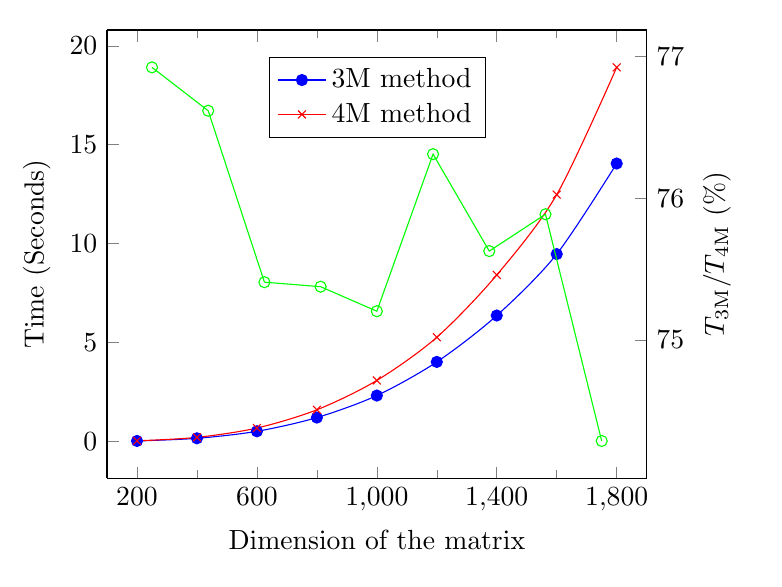
\begin{tikzpicture}
    \begin{axis}[xlabel={Dimension of the matrix},
                 ylabel={Time (Seconds)},
                 xmin=100,
                 xmax=1900,
                 xtick={200,600,1000,1400,1800},
                 minor x tick num=1,
                 axis y line*=left,
                 xlabel near ticks,
                 ylabel near ticks,
                 legend style={at={(0.3,0.85)},anchor=west}]
      \addplot[smooth,mark=*,blue] plot coordinates {
        ( 200, 0.01999700)
        ( 400, 0.15397700)
        ( 600, 0.50892300)
        ( 800, 1.20281700)
        (1000, 2.31664700)
        (1200, 4.01638900)
        (1400, 6.36303200)
        (1600, 9.46856100)
        (1800,14.04786400)
      };
      \addlegendentry{3M method}
      \addplot[smooth,color=red,mark=x] plot coordinates {
        ( 200, 0.02599600)
        ( 400, 0.20096900)
        ( 600, 0.67489700)
        ( 800, 1.59575800)
        (1000, 3.08053100)
        (1200, 5.26320100)
        (1400, 8.41372100)
        (1600,12.47710300)
        (1800,18.91012400)
      };
      \addlegendentry{4M method}
    \end{axis}
%
    \begin{axis}[hide x axis,
                 axis y line*=right,
                 ylabel={$T_{\text{3M}}/T_{\text{4M}}$ (\%)},
                 ylabel near ticks]
      \addplot[color=green,mark=o] plot coordinates {
        ( 200,76.923)
        ( 400,76.617)
        ( 600,75.408)
        ( 800,75.376)
        (1000,75.203)
        (1200,76.311)
        (1400,75.627)
        (1600,75.887)
        (1800,74.288)
      };
    \end{axis}
  \end{tikzpicture}
  \caption{Benchmark calculations of the 3M Method performed on Stallo
    (\url{https://www.notur.no/hardware/stallo}), using Hermitian matrix
    with elements as random numbers.}
  \label{fig-3M-speed}
\end{figure}

However, the numerical stability of the 3M Method needs to be taken care,
especially, for instance, if the real part is much larger than the imaginary
part\cite{Higham-SIAM-JMAA-13-681}
\begin{align}
  z&=x+\text{i}y=\left(\theta+\frac{\text{i}}{\theta}\right)^{2}
    =\theta^{2}-\frac{1}{\theta^{2}}+2\text{i},\\
  y&=\left(\theta+\frac{1}{\theta}\right)\left(\theta+\frac{1}{\theta}\right) %
    -\theta^{2}-\frac{1}{\theta^{2}}.
\end{align}

\subsection{Cholesky Decomposition}

\subsection{Eigenvalue Solver}

\begin{equation}
  \left(\mathbf{A}_{\text{R}}+\text{i}\mathbf{A}_{\text{I}}\right)%
    \left(\mathbf{X}_{\text{R}}+\text{i}\mathbf{X}_{\text{I}}\right)%
  =\left(\boldsymbol{\Lambda}_{\text{R}}+\text{i}\boldsymbol{\Lambda}_{\text{I}}\right)%
    \left(\mathbf{X}_{\text{R}}+\text{i}\mathbf{X}_{\text{I}}\right),
\end{equation}
is equivalent to
\begin{equation}
  \begin{bmatrix}
    \mathbf{A}_{\text{R}} & -\mathbf{A}_{\text{I}}\\
    \mathbf{A}_{\text{I}} & \mathbf{A}_{\text{R}}
  \end{bmatrix}
  \begin{bmatrix}
    \mathbf{X}_{\text{R}}\\
    \mathbf{X}_{\text{I}}
  \end{bmatrix}
  =\begin{bmatrix}
    \boldsymbol{\Lambda}_{\text{R}} & -\boldsymbol{\Lambda}_{\text{I}}\\
    \boldsymbol{\Lambda}_{\text{I}} & \boldsymbol{\Lambda}_{\text{R}}
  \end{bmatrix}
  \begin{bmatrix}
    \mathbf{X}_{\text{R}}\\
    \mathbf{X}_{\text{I}}
  \end{bmatrix},
\end{equation}

Suppose $\boldsymbol{\Lambda}$ is real, we have
\begin{equation}
  \begin{bmatrix}
    \mathbf{A}_{\text{R}} & -\mathbf{A}_{\text{I}}\\
    \mathbf{A}_{\text{I}} & \mathbf{A}_{\text{R}}
  \end{bmatrix}
  \begin{bmatrix}
    \mathbf{X}_{\text{R}}\\
    \mathbf{X}_{\text{I}}
  \end{bmatrix}
  =\begin{bmatrix}
    \boldsymbol{\Lambda}_{\text{R}} & \boldsymbol{0}\\
    \boldsymbol{0} & \boldsymbol{\Lambda}_{\text{R}}
  \end{bmatrix}
  \begin{bmatrix}
    \mathbf{X}_{\text{R}}\\
    \mathbf{X}_{\text{I}}
  \end{bmatrix}.
\end{equation}

\subsection{Linear Response Solver}

\begin{equation}
  \left(\mathbf{A}_{\text{R}}+\text{i}\mathbf{A}_{\text{I}}\right)%
    \left(\mathbf{X}_{\text{R}}+\text{i}\mathbf{X}_{\text{I}}\right)%
  =\left(\mathbf{B}_{\text{R}}+\text{i}\mathbf{B}_{\text{I}}\right)
\end{equation}
is equivalent to
\begin{equation}
  \begin{bmatrix}
    \mathbf{A}_{\text{R}} & -\mathbf{A}_{\text{I}}\\
    \mathbf{A}_{\text{I}} & \mathbf{A}_{\text{R}}
  \end{bmatrix}
  \begin{bmatrix}
    \mathbf{X}_{\text{R}}\\
    \mathbf{X}_{\text{I}}
  \end{bmatrix}
  =\begin{bmatrix}
    \mathbf{B}_{\text{R}}\\
    \mathbf{B}_{\text{I}}
  \end{bmatrix},
\end{equation}

% http://math.stackexchange.com/questions/166244/determinant-of-an-n-times-n-complex-matrix-as-an-2n-times-2n-real-determinan
\subsection{Determinant}

Let
\begin{equation}
  \mathbf{B}=\begin{bmatrix}
    \mathbf{A}_{\text{R}} & \text{i}\mathbf{A}_{\text{I}}\\
    \text{i}\mathbf{A}_{\text{I}} & \mathbf{A}_{\text{R}}
  \end{bmatrix},
\end{equation}
we have
\begin{equation}
  \det\mathbf{B}=\det\begin{bmatrix}
    \mathbf{A}_{\text{R}}+\text{i}\mathbf{A}_{\text{I}} & \text{i}\mathbf{A}_{\text{I}}\\
    \mathbf{A}_{\text{R}}+\text{i}\mathbf{A}_{\text{I}} & \mathbf{A}_{\text{R}}
  \end{bmatrix}
  =\det\begin{bmatrix}
    \mathbf{I} & \text{i}\mathbf{A}_{\text{I}}\\
    \mathbf{I} & \mathbf{A}_{\text{R}}
  \end{bmatrix}
  \det\begin{bmatrix}
    \mathbf{A}_{\text{R}}+\text{i}\mathbf{A}_{\text{I}} & \mathbf{0}\\
    \mathbf{0} & \mathbf{I}
  \end{bmatrix},
\end{equation}
and
\begin{equation}
  \det\begin{bmatrix}
    \mathbf{I} & \text{i}\mathbf{A}_{\text{I}}\\
    \mathbf{I} & \mathbf{A}_{\text{R}}
  \end{bmatrix}
  =\det\begin{bmatrix}
    \mathbf{I} & \text{i}\mathbf{A}_{\text{I}}\\
    \mathbf{0} & \mathbf{A}_{\text{R}}-\text{i}\mathbf{A}_{\text{I}}
  \end{bmatrix},
\end{equation}
hence
\begin{equation}
  \det\mathbf{B}=\det(\mathbf{A}_{\text{R}}-\text{i}\mathbf{A}_{\text{I}})
    \det(\mathbf{A}_{\text{R}}+\text{i}\mathbf{A}_{\text{I}})
  =\det\mathbf{A}\det\mathbf{A}^{\dagger}=|\det\mathbf{A}|^{2}.
\end{equation}

Moreover, if we let
\begin{equation}
  \mathbf{D}=\begin{bmatrix}
    \mathbf{I} & \mathbf{0}\\
    \mathbf{0} & \text{i}\mathbf{I}
  \end{bmatrix},
\end{equation}
we have
\begin{equation}
  \mathbf{D}^{-1}\mathbf{B}\mathbf{D}=\begin{bmatrix}
    \mathbf{A}_{\text{R}} & -\mathbf{A}_{\text{I}}\\
    \mathbf{A}_{\text{I}} & \mathbf{A}_{\text{R}}
  \end{bmatrix},
\end{equation}
and
\begin{equation}
  \det(\mathbf{D}^{-1}\mathbf{B}\mathbf{D})=\det\mathbf{B}=|\det\mathbf{A}|^{2}.
\end{equation}

\section{The Fortran 90 Adapter\index{Fortran 90 adapter}}
\label{section-F90-adapter}

To access the Fortran type in the C library \textsc{QcMatrix} is not trivial.
We take the strategy in Ref.~\cite{Pletzer-CSE-10-86}, by defining a Fortran
type with only one pointer member poiting to the Fortran matrix type \verb|LANG_F_MATRIX|.
As illustrated in Fig.~\ref{fig-F90-adapter-type}, the address of this defined
Fortran type \verb|matrix_ptr_t| can be saved in an integer array
\verb|f90_imat[SIZEOF_F_TYPE_P]| and accessed by the C function \verb|RealMatWrite|.
The convention between the integer array \verb|f90_imat[SIZEOF_F_TYPE_P]| and
the Fortran type \verb|matrix_ptr_t| can be done by the Fortran function
\verb|transfer|.
\begin{figure}[hbtp]
  \centering
  \includegraphics[width=17cm]{F90_adapter_type.pdf}
  \caption{Fortran 90 adapter for the external real matrix.}
  \label{fig-F90-adapter-type}
\end{figure}

Notice that the Fortran adapter subroutine is implemented in a module
\verb|f90_adapter|, the name mangling is taken care by CMake (see files
\verb|CMakeLists.txt| and \verb|cmake/f90_adapter.cmake|):
\begin{verbatim}
CMakeLists.txt:
IF(QCMATRIX_FC_MANGLING)
    INCLUDE(FortranCInterface)
    FortranCInterface_VERIFY()
    #FortranCInterface_VERIFY(CXX)
    FortranCInterface_HEADER(f90_mangling.h
                             MACRO_NAMESPACE "FC_"
                             SYMBOLS ${FC_MANGLING_SUB})
ENDIF()

cmake/f90_adapter.cmake:
IF(QCMATRIX_ENABLE_VIEW)
    SET(FC_MANGLING_SUB ${FC_MANGLING_SUB} f90_adapter:Mat_Ptr_Write)
ENDIF()
\end{verbatim}

In the C code of the Fortran adapter, we have:
\begin{verbatim}
/* uses CMake generated header file with auto-detected mangling */
#include "f90_mangling.h"

/* declaration of Fortran 90 subroutines */
... ...
#if defined(QCMATRIX_ENABLE_VIEW)
extern QVoid f90_adapter_Mat_Ptr_Write(QInt *iA,
                                       const QInt *len_mat_label,
                                       const QChar *mat_label,
                                       const QInt *view_option);
#endif
\end{verbatim}

\section{The Fortran 2003 Adapter\index{Fortran 2003 adapter}}
\label{section-F03-adapter}

In Fortran 2003, we can use the \verb|iso_c_binding| to facilitate the
access of Fortran type from the C code. As shown in Fig.~\ref{fig-F03-adapter-type},
the Fortran matrix type \verb|type(LANG_F_MATRIX)| pointer \verb|f_A|
can be converted from the C pointer \verb|type(C_PTR) A| using the function
\verb|c_f_pointer|. So that \textsc{QcMatrix} can access the Fortran matrix
type. Moreover, the name mangling is also taken care by \verb|iso_c_binding|.
\begin{figure}[hbtp]
  \centering
  \includegraphics[width=16cm]{F03_adapter_type.pdf}
  \caption{Fortran 2003 adapter for the external real matrix.}
  \label{fig-F03-adapter-type}
\end{figure}

\section{The Fortran 90 API\index{Fortran 90 API}}
\label{section-F90-API}

In contrast to the Fortran 90 adapter, the problem of API is how to access the
\verb|struct QcMat| in Fortran 90 code. In \textsc{QcMatrix}, we resort to the similar
strategy of the PETSc library (\url{http://www.mcs.anl.gov/petsc/}). As shown in
Fig.~\ref{fig-F90-API-type}, inside the \verb|type QcMat|, there is only an integer
(\verb|kind=SIZEOF_VOID_P| for offset) for saving the address of C \verb|struct|.
\begin{figure}[hbtp]
  \centering
  \includegraphics[width=16cm]{F90_api_type.pdf}
  \caption{Type convention in the \textsc{QcMatrix}Fortran 90 API.}
  \label{fig-F90-API-type}
\end{figure}

To be consistent with the \verb|type QcMat| defined in the Fortran API, the
\verb|struct QcMat_ptr| only has one member as the \verb|QcMat| pointer, so that
\verb|type QcMat| can be directly converted to \verb|struct QcMat_ptr|.

Again, the name mangling is taken care by CMake (file \verb|cmake/f90_api.cmake|):
\begin{verbatim}
IF(QCMATRIX_ENABLE_VIEW)
    SET(FC_MANGLING_SUB ${FC_MANGLING_SUB} f90_api_QcMatWrite)
ENDIF()
\end{verbatim}

\section{The Fortran 2003 API\index{Fortran 2003 API}}
\label{section-F03-API}

The use of \verb|iso_c_binding| also facilitates the Fortran 2003 API of \textsc{QcMatrix}.
As shown in Fig.~\ref{fig-F03-API-type}, the C pointer \verb|type(C_PTR)| can be directly
used in the Fortran code and passed to the C part, and converted to \verb|struct QcMat|.
\begin{figure}[hbtp]
  \centering
  \includegraphics[width=16cm]{F03_api_type.pdf}
  \caption{Type convention in the \textsc{QcMatrix}Fortran 2003 API.}
  \label{fig-F03-API-type}
\end{figure}

The name mangling can be solved by the declaration of the C function in the
\verb|interface| of the Fortran part and using the \verb|iso_c_binding|:
\begin{verbatim}
    interface
#if defined(QCMATRIX_ENABLE_VIEW)
        integer(C_INT) function f03_api_QcMatWrite(A, mat_label, view_option) &
            bind(C, name="f03_api_QcMatWrite")
            use iso_c_binding
            type(C_PTR), intent(in) :: A
            character(C_CHAR), intent(in) :: mat_label(*)
            integer(C_INT), value, intent(in) :: view_option
        end function f03_api_QcMatWrite
#endif
    end interface
\end{verbatim}

\section{Procedure of \texttt{QcMatSetExternalMat}\index{\texttt{QcMatSetExternalMat}}}
\label{section-procedure-QcMatSetExternalMat}

The function \verb|QcMatSetExternalMat| involves conventions of different
matrix types in the API and adapter parts, which are illustrated in Fig.~\ref{fig-F90-QcMatSetExternalMat}
and Fig.~\ref{fig-F03-QcMatSetExternalMat} respectively for the Fortran 90 and 2003.
\begin{figure}[hbtp]
  \centering
  \includegraphics[width=16cm]{F90_QcMatSetExternalMat.pdf}
  \caption{Procedure of \texttt{QcMatSetExternalMat} (Fortran 90).}
  \label{fig-F90-QcMatSetExternalMat}
\end{figure}

\begin{figure}[hbtp]
  \centering
  \includegraphics[width=16cm]{F03_QcMatSetExternalMat.pdf}
  \caption{Procedure of \texttt{QcMatSetExternalMat} (Fortran 2003).}
  \label{fig-F03-QcMatSetExternalMat}
\end{figure}

It should be noticed that the context of the external matrix \verb|A_ext| will not
be destroyed by \verb|QcMatDestroy|. So that the \verb|QBool external_mat| has been
introduced to indicate if the \linebreak\verb|QInt f90_imag[SIZEOF_F_TYPE_P]| or
\verb|QVoid *f03_mat| points to an external matrix.

\section{Procedure of \texttt{QcMatGetExternalMat}\index{\texttt{QcMatGetExternalMat}}}
\label{section-procedure-QcMatGetExternalMat}

The function \verb|QcMatGetExternalMat| also involves the conventions of different
matrix types in the API and adapter parts, which are illustrated in Fig.~\ref{fig-F90-QcMatGetExternalMat}
and Fig.~\ref{fig-F03-QcMatGetExternalMat} respectively for the Fortran 90 and 2003.
\begin{figure}[hbtp]
  \centering
  \includegraphics[width=16cm]{F90_QcMatGetExternalMat.pdf}
  \caption{Procedure of \texttt{QcMatGetExternalMat} (Fortran 90).}
  \label{fig-F90-QcMatGetExternalMat}
\end{figure}

\begin{figure}[hbtp]
  \centering
  \includegraphics[width=16cm]{F03_QcMatGetExternalMat.pdf}
  \caption{Procedure of \texttt{QcMatGetExternalMat} (Fortran 2003).}
  \label{fig-F03-QcMatGetExternalMat}
\end{figure}

% files and directories of QcMatrix
\chapter{Files and Directories of \textsc{QcMatrix}}
\label{chapter-files}

\begin{enumerate}
  \item \verb|AUTHORS|: Author information.
  \item \verb|ChangeLog|: Changes made.
  \item {\color{blue}\verb|cmake|} and \verb|CMakeLists.txt|: CMake files.
  \item \verb|COPYING| and \verb|COPYING.LESSER|: The license.
  \item {\color{blue}\verb|doc|}
    \begin{enumerate}
      \item {\color{blue}\verb|figures|}: Figures.
      \item {\color{blue}\verb|logo|}: Logos.
      \item \verb|manual.pdf|, \verb|manual.tex| and \verb|refs.bib|: Manual files.
      \item \verb|tutorial.pdf| and \verb|tutorial.tex|: Tutorial files.
    \end{enumerate}
  \item {\color{blue}\verb|examples|}: Examples for tutorial.
  \item {\color{blue}\verb|include|}: Header files.
    \begin{enumerate}
      \item {\color{blue}\verb|adapter|}: Header files for the adapters of %
        external libraries.
      \item {\color{blue}\verb|api|}: Header files of APIs.
      \item {\color{blue}\verb|impls|}: Header files of implemented matrices %
        in \textsc{QcMatrix}.
      \item {\color{blue}\verb|lapack|}: Header files for calling BLAS and %
        LAPACK libraries, used by internal real matrix library and test suite.
      \item \verb|qcmatrix.h|: Header file of \textsc{QcMatrix} C APIs.
      \item \verb|README|: Some rules for these header files.
      \item {\color{blue}\verb|tests|}: Header files of test suite.
      \item {\color{blue}\verb|types|}: Header files of basic and matrix types %
        used in \textsc{QcMatrix}.
      \item {\color{blue}\verb|utilities|}: Header files of utilities.
    \end{enumerate}
  \item \verb|INSTALL|: Installation instruction.
  \item {\color{blue}\verb|maintenance|}: Maintenance files.
  \item \verb|MANIFEST.in|: Python manifest template for source distribution.
  \item \verb|NEWS|: List of user-visible changes.
  \item \verb|PKG-INFO|: PKG-INFO metadata file.
  \item {\color{blue}\verb|QcMatrix|}: Python files.
  \item \verb|qcmatrix.bib|: \textsc{QcMatrix} citation.
  \item \verb|README|: A very important file ;-).
  \item \verb|RULES|: Rules for contribution.
  \item \verb|setup.cfg|: Python setup configuration file.
  \item {\color{green}\verb|setup.py|}: Python setup script.
  \item {\color{blue}\verb|src|}
    \begin{enumerate}
      \item {\color{blue}\verb|adapter|}: Source codes of adapters.
      \item {\color{blue}\verb|cmplx_mat|}: Source codes of complex matrix.
      \item {\color{blue}\verb|qcmat|}: Source codes of square block complex matrix.
        \begin{enumerate}
          \item {\color{blue}\verb|c|}: Source codes of APIs \verb|QcMatGetExternalMat| %
            and \verb|QcMatSetExternalMat|.
          \item {\color{blue}\verb|f03|}: Source codes of Fortran APIs (using
            Fortran 2003 functionalities).
          \item {\color{blue}\verb|f90|}: Source codes of Fortran APIs (using
            Fortran 90 functionalities).
          \item {\color{blue}\verb|tests|}:  Source codes of APIs for tests only.
        \end{enumerate}
      \item {\color{blue}\verb|real_mat|}: Source codes of real matrix.
      \item {\color{blue}\verb|xray|}: Source codes of X-ray spectroscopies.
    \end{enumerate}
  \item {\color{blue}\verb|tests|}
    \begin{enumerate}
      \item {\color{blue}\verb|c|}: Source codes of C test suite.
        \begin{enumerate}
          \item {\color{blue}\verb|adapter|}: A simple external C matrix library %
            (indeed it just \textsc{QcMatrix} source codes themselves, but to be %
            compiled here to mimic the external C matrix library).
            \begin{enumerate}
              \item {\color{green}\verb|clean_c_adapter.sh|}: Script for cleaning %
                the files created by {\color{green}\verb|init_c_adapter.sh|}.
              \item {\color{blue}\verb|cmake|} and \verb|CMakeLists.txt|: CMake files.
              \item {\color{blue}\verb|include/impls|}: Header files.
              \item {\color{green}\verb|init_c_adapter.sh|}: Script for copying files %
                from \textsc{QcMatrix} for this external C matrix library.
              \item \verb|README|: Please follow this file to compile this external %
                C matrix library.
            \end{enumerate}
          \item {\color{blue}\verb|api|}: Source codes of testing \textsc{QcMatrix} %
            C APIs.
        \end{enumerate}
      \item {\color{blue}\verb|f90|}: Source codes of Fortran test suite.
        \begin{enumerate}
          \item {\color{blue}\verb|adapter|}: A simple external Fortran matrix library.
            \begin{enumerate}
              \item {\color{green}\verb|clean_f_adapter.sh|}: Script for cleaning %
                the files created by {\color{green}\verb|init_f_adapter.sh|}.
              \item \verb|CMakeLists.txt|: CMake file.
              \item {\color{green}\verb|init_f_adapter.sh|}: Script for copying files %
                from \textsc{QcMatrix} for this external Fortran matrix library.
              \item \verb|README|: Please follow this file to compile this external %
                Fortran matrix library.
              \item {\color{blue}\verb|src|}: Source codes of this external Fortran %
                matrix library.
            \end{enumerate}
          \item {\color{blue}\verb|api|}: Source codes of testing \textsc{QcMatrix} %
            Fortran APIs.
          \item \verb|test_3M_method.F90|: Source code for testing the efficiency of %
            3M method for complex matrix-matrix multiplication.
          \item \verb|timer.F90|: Source code recording the CPU time, needed by %
            \verb|test_3M_method.F90|.
        \end{enumerate}
    \end{enumerate}
  \item \verb|TODO|: Todo list.
  \item {\color{blue}\verb|tools|}: Tools for \textsc{QcMatrix}.
\end{enumerate}

% limitations
\chapter{Limitations of \textsc{QcMatrix}}
\label{chapter-limitations}

\begin{enumerate}
  \item Chapters~\ref{chapter-SCF-solvers}, \ref{chapter-RSP-solvers}, \ref{chapter-xray}
    and \ref{chapter-molecular-electronics}, Sections~\ref{section-QcMat} and \ref{section-complex-matrix}
    to be finished.
  \item Only the real matrix adapter has been tested.
  \item Reading ASCII format file is not tested.
  \item C++ and Python adapters and APIs to be implemented.
  \item The parallelization is not implemented in \textsc{QcMatrix}, but relies
    on the external matrix libraries.
  \item Internal C real matrix may not be efficient, and is not parallelized.
  \item Only one type of adapter can be compiled (C, C++ or Fortran) at once.
  \item We do not guarantee that \textsc{QcMatrix} will always check the validity
    of all input arguments, users should be more careful on sending correct
    arguments to \textsc{QcMatrix}.
  \item There will be some compiler warnings if HDF5 library is used.
  \item There is also a bug regarding the use of HDF5 library: if \textsc{QcMatrix}
    does not use HDF5 library, but the external matrix library does, then it
    may have error when linking the \textsc{QcMatrix} test suite as executables.
\end{enumerate}

% back end
\backmatter

% references
\begin{small}
  \bibliographystyle{unsrt}
%  \bibliographystyle{abbrv}
  \bibliography{refs}
\end{small}

% index
\printindex

\end{document}
